\section{ERRORR}
\label{sERRORR}
\index{ERRORR|textbf}

\hypertarget{sERRORRhy}{The}
ERRORR module is used to produce cross section and distribution
covariances from error files in ENDF format.

This chapter describes the ERRORR module in NJOY2016.0.

\subsection{Introduction}
\label{ssERRORR_Intro}

After evaluators have completed their review of the available
measurements of various nuclear data (having true values $\sigma_{1},
\sigma_{2}, \sigma_{3},\cdots$) and the theoretical analysis, they will
have formed at least a subjective opinion of the joint probability
distribution of the data examined; that is, the probability
\[ P(\sigma_{1},\sigma_{2},\cdots) \, d\sigma_{1}\, d\sigma_{2}\cdots\]
that the true value of $\sigma_1$ lies in the range $(\sigma_1,
\sigma_1 {+} d\sigma_1)$, and that $\sigma_2$ lies in the range
$(\sigma_2, \sigma_2 {+} d\sigma_2)$, etc.  In the early versions
of the ENDF format, only the first moments (expectation values) of this
probability distribution could be included in the numerical data
files.  However, beginning with ENDF/B-IV and expanding significantly
in ENDF/B-V and later, the second moments of the data
probability distributions have been included in many of the files.
As discussed in Section~\ref{ssERRORR_Defs}, these second moments
(or ``data covariances'')
contain information on the uncertainty of individual data, as well as
correlations that may exist.  Fig.~\ref{b10cov} shows an example of
this for $^{10}$B from ENDF/B-VII.0.  The top plot shows the first
moment (the percent standard deviation) of the uncertainty in the
(n,$\alpha$) cross section.  The right-hand plot shows the cross
section.  The center plot shows the correlations between the
(n,$\alpha$) cross section at one energy to itself at other energies.
\index{covariances}

\begin{figure}[thb]\centering
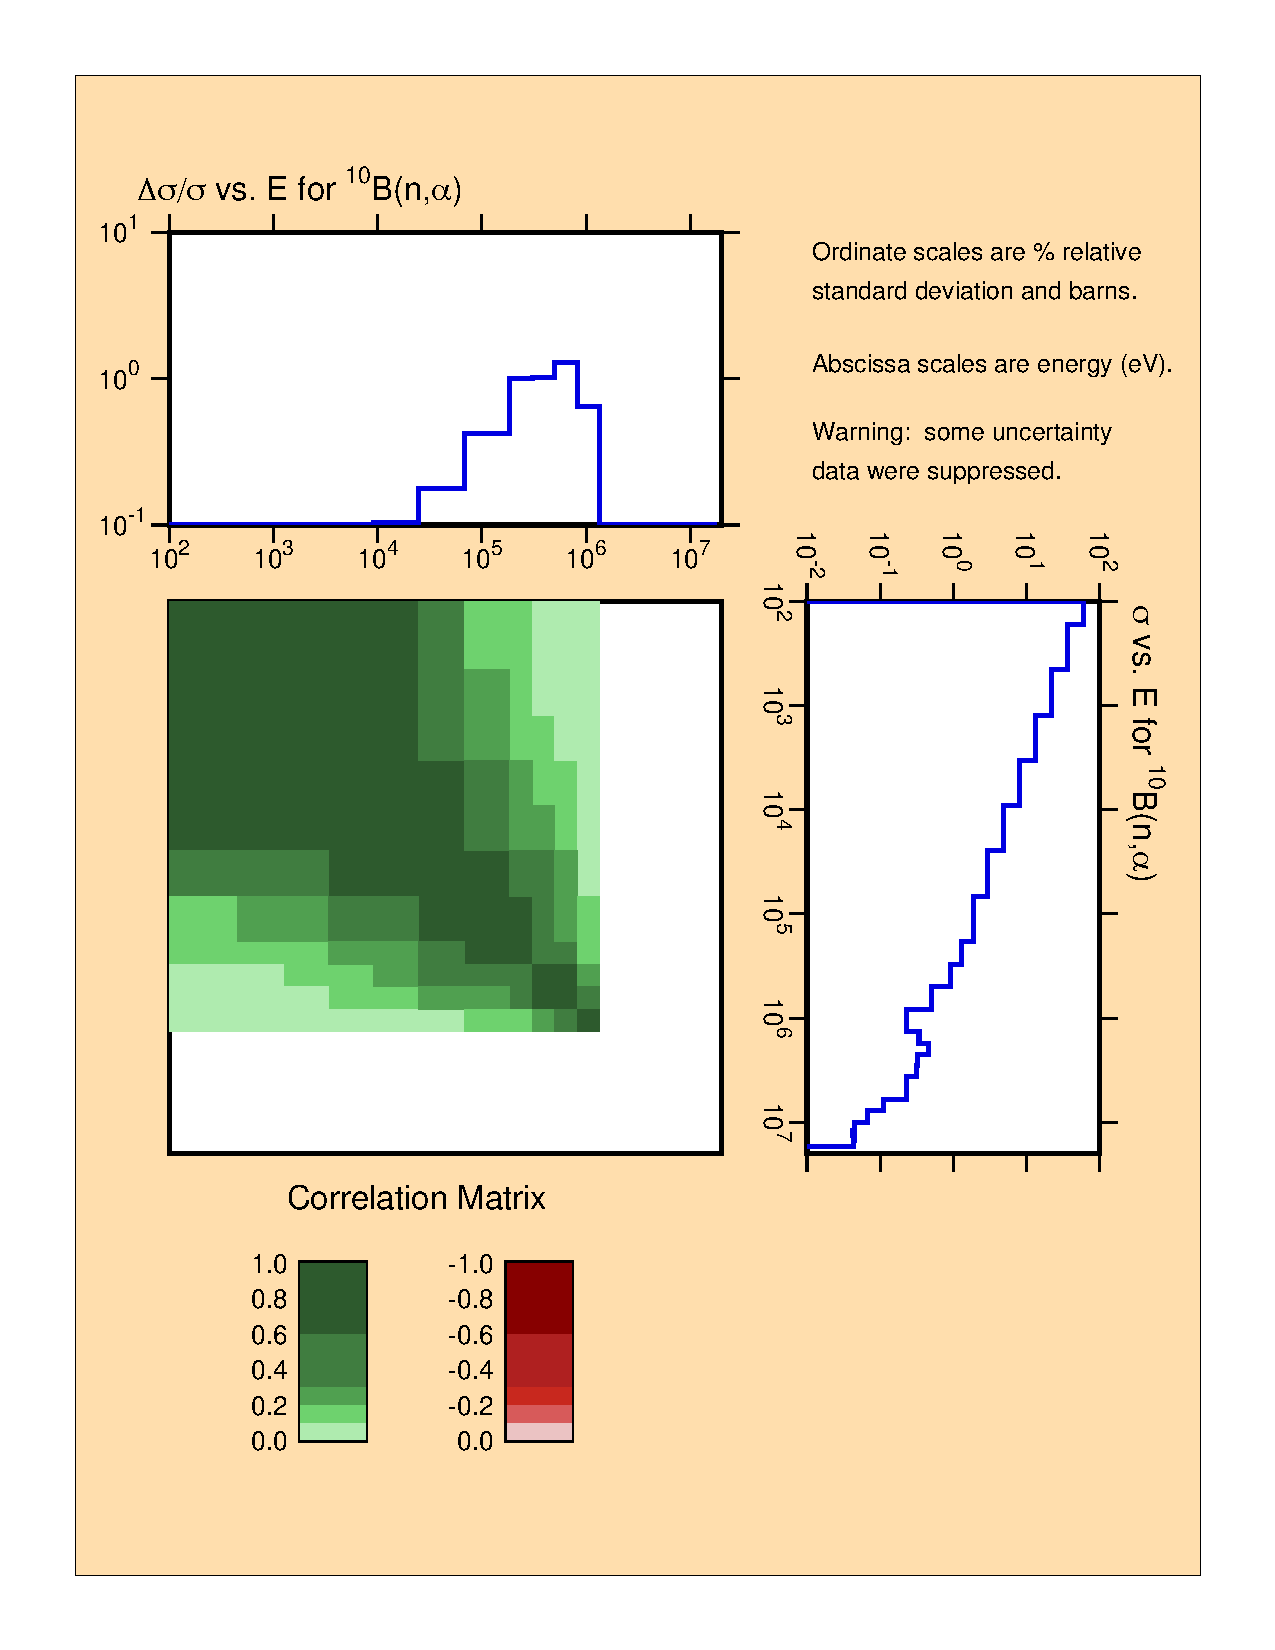
\includegraphics[keepaspectratio, width=5.0in,angle=0]{figs/b10covack}
\caption[ENDF/B-VII.0 $^{10}$B(n,$\alpha$) covariance data]{Covariance
 plot for $^{10}$B(n,$\alpha$) from ENDF/B-VII.0.  This reaction is used as
 a standard in the ENDF system.}
\label{b10cov}
\end{figure}

Data covariances have many applications.  For example, they can be
combined with sensitivity coefficients to obtain the uncertainty, due
to the data, in calculated quantities of applied interest\cite{Gerstl}.
This information can be used in turn to judge the adequacy of the data
for that application.
\index{sensitivity analysis}

The availability of data covariances also makes it possible to use the
generalized method of least squares to improve the data evaluation
after new integral or differential measurements have been
performed\cite{Reupke}.  The least-squares method requires only data
covariances (not the full probability distribution), and the improved,
or adjusted, data are guaranteed\cite{Hamilton} to have the smallest
possible uncertainties, regardless of the actual shape of the underlying
probability distribution function, $P(\sigma_1, \sigma_2,\cdots)$.
\index{data adjustment}
Thus, the ENDF-formatted covariance files contain, in about as compact
a form as possible, a statement about the quality of the data, as well
as sufficient information (in principle) to carry out future
improvements on an objective basis.

In many of these applications, it is necessary to begin by converting
energy-dependent covariance information in ENDF format\cite{ENDF102}
into multigroup form.  This task can be performed conveniently in the
NJOY environment, using the ERRORR module.  In particular,
ERRORR calculates the uncertainty in infinitely dilute multigroup cross
sections (or multigroup $\bar{\nu}$ values), as well as the associated
correlation coefficients.  These data are obtained by combining
absolute or relative covariances from ENDF Files 31, 32, 33, 34, 35 and 40
with multigroup $\bar{\nu}$ data, cross section data, angular disbribution
data, fission spectra data or radionuclide production data.  These
multigroup data are obtained from \hyperlink{sGROUPRhy}{GROUPR}
processing, or in some instances are calculated
within ERRORR.  ERRORR is coded to treat all approved ENDF-4, -5, and -6
covariance formats for these files.  ERRORR can also treat
resolved-resonance covariances given in File 32 using the old
Breit-Wigner resolved-resonance parameter uncertainties (\cword{LRF}=1
and \cword{2}) in Version-5 format, the ``Version-5 compatible''
option of Version 6 (\cword{LCOMP}=0) using the new formats
that include resonance-resonance covariances, and the newest
format based on Reich-Moore-Limited parameters that include
resonance-resonance correlations between different reactions.

The methodology of ERRORR assumes that the weighting flux
\index{weighting flux} used to convert energy-dependent cross sections
into multigroup averages is free of uncertainty.  In cases in which
the cross-section information is obtained from an existing multigroup
library, it is usually necessary to make assumptions about the shape
of the cross section and the weight function within certain input
energy groups.

\subsection{Definitions of Covariance-Related Quantities}
\label{ssERRORR_Defs}

For convenient reference in discussing the methodology and input
requirements of the ERRORR module, we next review the basic definitions
of covariance-related quantities.  Let $x_{0}$ and $y_{0}$ be the
evaluated values of $x$ and $y$, respectively:

\begin{equation}
   x_{0} \equiv {\rm E}[x] \; ,
\end{equation}

\noindent
and

\begin{equation}
   y_0 \equiv {\rm E}[y] \; .
\end{equation}

\noindent
Here E is the expectation operator, which performs an average over the
joint probability distribution of $x$ and $y$.  The second moment of
this distribution is called the covariance of $x $ with $y$:

\begin{equation}
{\rm cov} (x,y) \equiv {\rm E}[(x\;-\;x_0)\;(y\;-\;y_0)]\;.
\label{cov}
\end{equation}

\noindent
Covariance is a measure of the degree to which $x$ and $y$ are both
affected by the same sources of error.  The covariance of $x$ with
itself is called the variance of $x$:

\begin{equation}
{\rm var}(x) \equiv {\rm cov}(x,x) = {\rm E}[(x\;-\;x_0)^2]\;.
\end{equation}

\noindent
The more familiar standard deviation $\Delta x$ (also called the
``uncertainty'') is simply

\begin{equation}
\Delta x \equiv [{\rm var} (x)]^{1/2} = [{\rm cov}(x,x)]^{1/2} \; .
\label{deltax}
\end{equation}

\noindent
The correlation between $x$ and $y$ (also called the correlation
coefficient) is defined as

\begin{equation}
{\rm corr}(x,y) \equiv \frac{{\rm cov}(x,y)}{\Delta x\;\Delta y} \;.
\label{corr}
\end{equation}

\noindent
The absolute value of a correlation coefficient is guaranteed to be
less than or equal to unity.  Another useful quantity is the relative
covariance of $x$ with $y$,

\begin{equation}
{\rm rcov}(x,y) \equiv \frac {{\rm cov}(x,y)}{x_0 \; y_0} \;.
\label{rcov}
\end{equation}

\noindent
Unlike ${\rm cov}(x,y)$, the relative
{\rm cov}ariance ${\rm rcov}(x,y)$ is a dimensionless quantity.
Closely related to the relative covariance is the relative standard
deviation,

\begin{equation}
\frac {\Delta x}{x_0} \;=\; \frac {[{\rm cov}(x,x)]^{1/2}}{x_0} \;,
\end{equation}

\noindent
which, from Eq.~\ref{rcov}, can be written as

\begin{equation}
\frac {\Delta x}{x_0}\; =\; [{\rm rcov}(x,x)]^{1/2} \; .
\label{deltax0}
\end{equation}

\noindent
Combining Eqs.~\ref{corr} and \ref{rcov}, we have another useful result,

\begin{equation}
{\rm corr}(x,y) = \frac{{\rm rcov}(x,y)}{(\Delta x/x_0) (\Delta y/y_0)}\;.
\label{corr2}
\end{equation}

While it is customary to speak of uncertainties\index{uncertainties}
and correlations\index{correlations} as separate entities, these
are actually just two different aspects of the covariance.  If one
has a set of absolute covariances for various reactions, including
the self-covariance, then Eqs.~\ref{deltax} and \ref{corr} can be used
to calculate $\Delta x$ and corr$(x,y)$.  Similarly, if one has a set
of relative covariances, one can use Eqs.~\ref{deltax0} and
\ref{corr2} to calculate $\Delta x/x_0$ and corr$(x,y)$.

Consider now a set of nuclear data $\sigma_i$ with uncertainties
characterized by the covariances {\rm cov}$(\sigma_i,\sigma_j)$.  Let
$A$ and $B$ be two linear functions of the $\sigma_i$,

\begin{equation}
A =\sum_{i} \; a_i \; \sigma_i
\end{equation}

\noindent
and

\begin{equation}
B =\sum_{j} \; b_j \; \sigma_j \; ,
\end{equation}

\noindent
where the $a_i$ and $b_j$ are sets of known constants.  The above
definitions can be used to calculate the covariances of the functions
$A$ and $B$ induced by the covariances of the data.
From Eq.~\ref{cov},

\begin{eqnarray} {\rm cov}(A,B) & = & {\rm E} \left\{ {\vphantom{\sum_j}}\left
({\vphantom{\sum_j}}\sum_{i} \; a_i \; \sigma_i \; - \;\sum_{i}\; a_i {\rm E}
(\sigma_i)\right)\;{\vphantom{\sum_j}}\left(\sum_{j} \;b_j \;\sigma_j - \sum_{j}
(\sigma_j )\right )\right \} \nonumber \\
 & = & \sum_{i,\; j} \; a_i \; b_j \; {\rm E} \left \{ {\vphantom{\sum}}\left
({\vphantom{\sum}}\sigma_i
 {-}  {\rm E} (\sigma_i)  \right ) \;
 \left ({\vphantom{\sum}} \sigma_j{-}{\rm E} (\sigma_j) \right)  \right \}  \;,
\end{eqnarray}

\noindent
so that

\begin{equation}
{\rm cov}(A,B) = \sum_{i,\,j} \; a_i \; b_j \; {\rm cov}(\sigma_i , \sigma_j ) \
\label{e11}
\end{equation}

\noindent
This result, called the ``propagation of errors'' formula, is
fundamental to the subject of multigroup processing of ENDF covariance
data and will be referenced frequently in later sections of this
chapter.

\subsection{Structure of ENDF Files 31, 33, and 40: Energy-Dependent Data}
\label{ssERRORR_Str}

Data in ENDF format are stored in various numbered ``files,'' where the
file number depends on the type of information contained.  For example,
the covariances of $\bar{\nu}(E)$ (the average number of neutrons per
fission, which is a function of the incident neutron energy) are stored
in File 31, where the possible ``reaction'' types are prompt
$\bar{\nu}$, delayed $\bar{\nu}$, and total $\bar{\nu}$.  File 33
contains the covariances of energy-dependent cross sections.  In
general, for data given in File N, covariance data are given in
File (N+30).  The structures of Files 31, 33, and 40 are identical
and will be described first.

Files 31, 33, and 40 describe the covariances of energy-dependent data.  To
expand on this point, we recall that the full energy dependence of a
cross section $\sigma (E)$, for example, is described in the ENDF File
3 by specifying the cross-section values at a relatively small number
of energy points and then providing a set of interpolation laws to be
used in reconstructing the actual cross section at any intermediate
energy.  Somewhat the same philosophy is used to describe the
two-dimensional energy dependence of data covariances in Files 31, 33, and
40.  That is, one specifies a set of numerical data and a set of
formulae, which together can be used to compute ${\rm cov}(x,y)$ for
any desired pair of energies, $E_x$ and $E_y$.  Although
the interpolation laws are presently restricted to the simple forms
described below, it is not true (as sometimes stated) that ENDF
contains multigroup covariances.  The expression ``multigroup
covariance'' refers to the covariance of one multigroup-averaged
quantity with another averaged quantity, whereas ENDF contains the
covariances between point-energy data.  It is precisely the task of
ERRORR to compute multigroup covariances, starting from point
covariances.

Files 31, 33, and 40 of an evaluation for material \cword{MAT} are divided
into ``sections,'' indexed by the reaction type \cword{MT}.  A section
\cword{(MAT,MT)} is further subdivided into ``subsections.''  As
described in the ENDF formats manual, a subsection is the repository
for all explicit statements of the two-dimensional energy dependence
of the covariances of reaction \cword{(MAT,MT)} with another reaction
\cword{(MAT1,MT1)}.  Because covariances are symmetric, a subsection
with \cword{MAT1}=\cword{MAT} and \cword{MT1}$<$\cword{MT} would be
redundant with a subsection in an earlier section, and such data are,
by convention, omitted from the ENDF files.

Subsections are further divided into ``sub-subsections.''  Two different
types of sub-subsections are used in the ENDF-5 and ENDF-6 formats.  ERRORR
also treats data covariances in the earlier
ENDF-4 format, but this is of little practical interest since only three
covariance evaluations were released in the Version-4 format.  ``NI-type''
sub-subsections are used to express covariances explicitly, while
``NC-type'' sub-subsections are used to indicate the existence of
connections between various data that result in ``implicit'' covariance
contributions for various reaction pairs.  We shall return to this
point when discussing NC-Type Sub-Subsections.

\paragraph{NI-Type Sub-Subsections.} Multiple NI-type sub-subsections
are used to describe multiple, statistically independent sources of
uncertainty for a given reaction pair.  If $ {\rm cov}(x,y)_n$ is the
covariance computed from the data in one sub-subsection, then, because
the uncertainties in different sub-subsections are uncorrelated,
$$
{\rm cov}(x,y) \;= \; \sum^{{\rm NI}}_{n=1} \; {\rm cov}(x,y)_n \; ,
$$
\vspace{2 pt}
where NI is the number of NI-type sub-subsections in the current
subsection.\ The numerical content of one NI-type sub-subsection
consists of either one or two energy grids, a collection of constants,
and a parameter \cword{LB}.  The parameter \cword{LB} governs how the
energies and constants are to be used in constructing the covariance in
various rectangular regions of $E_x {-}E_y$ space.  For \cword{LB}=0, 1,
2 and 8, a single table containing pairs $(E_i,F_i)$ is
given.  For \cword{LB}=3 and \cword{LB}=4, two such tables are given.  For
\cword{LB}=5,  a single set of energies $E_i$ is given, along with an
associated square matrix of constants $G_{ij}$.  Finally, for
\cword{LB}=6, two energy grids are given, along with an associated
rectangular matrix of constants $G'_{ij}$.

The first of these tables $(E_i,F_i)$ defines a function $f(E)$
that is constant except for
discrete steps at energies $E_i$,

\begin{equation}
f(E) = F_i ,\;{\rm if}\; E_i{\leq} E{<}E_{i+1} \;.
\label{e12}
\end{equation}
\vspace{0.5 pt}

\noindent
Similarly, if there is a second table,

\begin{equation}
f'(E) = F'_j , \; {\rm if}\; E'_j{\leq}E{<}E'_{j+1} \;.
\end{equation}
\vspace{0.5 pt}

\noindent
The \cword{LB}=5 matrix data $G_{ij}$ also define a function,

\begin{equation}
g(E_x,E_y) = G_{ij},\, {\rm{if}}\; E_i {\leq} E_x{<}E_{i+1} \;{\rm {and}}\; E_j
\; , \end{equation}

\noindent
and similarly for \cword{LB}=6

\begin{equation}
g'(E_x,E_y) = G'_{ij}, \, {\rm {if}}\;  E_i  {\leq} E_x {<} E_{i+1}\;{\rm {and}}
{\leq} E_y{<}E'_{j+1} \;.
\end{equation}
\vspace{1 pt}

\noindent
These functions are simply histograms in either one or two dimensions.
Using the functions $f$, $f'$, $g$, and $g'$ thus defined, we can list
the formulae in Eq.~\ref{lbopts}, which are used to specify energy-dependent
covariances for the different allowed values of \cword{LB}.  Thus, if
$x$ is the value of the cross section or of the $\bar{\nu}$ value for the
reaction \cword{(MAT,MT)} that determines the ENDF/B
\underline{section}, and if $y$ is the value for the reaction
\cword{(MAT1,MT1)} that determines the \underline{subsection}, then for

\begin{equation}
\begin{array} {rrrll}
{\rm {LB}} & = & 0, &  {\rm {{\rm cov}}} (x,y)_n   & = \; f (E_x) \,
  \delta (E_x,E_y)   \\
{\rm {LB}} & = & 1, &  {\rm {r{\rm cov}}} (x,y)_n  & =  \; f (E_x) \,
  \delta (E_x,E_y)  \\
{\rm {LB}} & = & 2, &  {\rm {r{\rm cov}}} (x,y)_n  & =  \; f (E_x)\,f(E_y)  \\
{\rm {LB}} & = & 3, &  {\rm {r{\rm cov}}} (x,y)_n  & =  \;f (E_x)\,f'(E_y) \\
{\rm {LB}} & = & 4, &  {\rm {r{\rm cov}}} (x,y)_n  & = \; f (E_x) \,
  \delta (E_x,E_y)\;f'(E_x)\,f'(E_y)
\\ {\rm {LB}} & = & 5, &  {\rm {r{\rm cov}}} (x,y)_n  & =  \;g (E_x,E_y)  \\
{\rm {LB}} & = & 6, &  {\rm {r{\rm cov}}} (x,y)_n  & = \; g'(E_x,E_y)\,\,.
\end{array}
\label{lbopts}
\end{equation}

\noindent
The symbol $\delta (E_x,E_y)$ has the following meaning: $\delta
(E_x,E_y){ =} 1$ if $E_x$ and $E_y$ fall in the same energy interval of
the first table $(E_i$, $F_i$), and $\delta(E_x,E_y){ =} 0$ otherwise.

The final covariance law, \cword{LB}=8, is an exceptional case that
cannot be expressed in terms of point covariances.  \cword{LB}=8 is
used primarily to represent uncertainty effects due to suspected, but
unresolved, energy-dependent structure in a given cross section.  If
$\Delta E_j$ is the energy width of the $j$-th ``union'' energy group
(see the discussion of union groups in Section~\ref{ssERRORR_UnionGrid}),
and if this group
lies within the $k$-th range ($E_k, E_{k+1}$) of an ENDF \cword{LB}=8
energy grid, then the effect of the \cword{LB}=8 subsection is to
trigger the addition of an uncorrelated contribution of
$F_k\,(E_{k+1} - E_k )/\Delta E_j$ to the (absolute) variance
of the $j$-th union-group cross section.  No contributions to
off-diagonal elements of the multigroup covariance matrix are
generated by an \cword{LB}=8 sub-subsection.

\paragraph{NC-Type Sub-Subsections.} NC-type sub-subsections, which
describe covariances indirectly, are used in several evaluation
situations, which are flagged by different values of the parameter
\cword{LTY}.  The first situation, \cword{LTY}=0, occurs when the
following two conditions are met:  (a) the covariances of a given
reaction \cword{MT}, both with itself and with other reactions, can be
deduced in an energy range \cword{(E1, E2)} solely from the application
of a cross-section ``derivation relation,''

\begin{equation}
x({\mathtt{MAT,MT}};E) = \sum_{i} \; C_i \; x({\mathtt{MAT,MT}}_i; E),\;
\label{e17}
\end{equation}

\noindent
and (b) the covariances of all of the reaction cross sections on the
right-hand side of Eq.~\ref{e17} have been given directly (that is, using
only NI-type sub-subsections) throughout the range (\cword{E1, E2}).
The energy boundaries \cword{E1} and \cword{E2}, the constants $C_i$,
and the reaction identifiers \cword{MT}$_i$ are specified in an NC-type
sub-subsection with \cword{LTY}=0.  This format is widely used in the
ENDF/B library, and it makes possible the elimination of large volumes
of otherwise redundant data.  It also introduces considerable
complexity in the multigroup processing, as discussed in
Section~\ref{ssERRORR_UnionGrid}, and
adds to the computer running times. The presence of this one short
sub-subsection affects the calculation of the covariances for many
different reaction pairs, such as $x$\cword{(MAT,MT)} with
$x$\cword{(MAT,MT}$_i$\cword{)}.  Less widely used are NC-type
sub-subsections with \cword{LTY}=1.  These are employed when a reaction
\cword{MT} in material \cword{MAT} is evaluated in some energy range
\cword{(E1, E2)} as a ratio to a standard reaction \cword{MTS} in some
other material \cword{MATS}.  That is,

\begin{equation}
x({\mathtt{MAT,MT}};E) = R(E)\, x ({\mathtt{MATS,MTS}};E).
\label{e18}
\end{equation}

In practical evaluation situations, the uncertainty of $R$ is almost
never correlated with that of $x$\cword{(MATS,MTS)}.  Because of this,
the relative uncertainty in $R$ is treated simply as one independent
component of the relative uncertainty in $x$\cword{(MAT,MT)}, and it is
described using normal NI-type sub-subsections.  On the other hand, the
contribution from uncertainty in $x$\cword{(MATS,MTS)} is represented
with an NC-type sub-subsection with \cword{LTY}=1, which contains,
in ENDF/B-V, only \cword{E1}, \cword{E2}, \cword{MATS}, and \cword{MTS}.
The actual numerical covariance information must be read from the
evaluation for the standard material \cword{MATS}, which usually resides
on an entirely different ENDF tape.  An NC-type sub-subsection with
\cword{LTY}=1, which occurs in a given subsection
\cword{(MAT,MT; MAT,MT)}, affects the calculation of the covariances
only for the current reaction pair (reaction \cword{MT} with itself)
and, in this respect, is more like an NI-type sub-subsection than, for
example, an NC-type sub-subsection with \cword{LTY}=0.  This similarity
is exploited in the processing of ratio covariances, as discussed in
Section~\ref{ssERRORR_Ratio}.

An NC-type sub-subsection with \cword{LTY}=2 is used, in a similar way,
to describe the covariances of $x$\cword{(MAT,MT)} with
$x$\cword{(MATS,MTS)}.  As in the \cword{LTY}=1 case, an \cword{LTY}=2
sub-subsection contains only \cword{E1}, \cword{E2}, \cword{MATS}, and
\cword{MTS}.

An NC-type sub-subsection with \cword{LTY}=3 is included in material
\cword{MATS} to describe the (redundant) covariances of
$x$\cword{(MATS,MTS)} with $x$\cword{(MAT,MT)}.  The numerical
information contained here is the same as for \cword{LTY}=1 and
\cword{LTY}=2.  As discussed in Section~\ref{ssERRORR_Ratio},
an important function of
\cword{LTY}=3 data is to help locate reactions other than
\cword{(MAT,MT)} that have been measured relative to the same standard
\cword{(MATS,MTS)}.


\subsection{Resonance-Parameter Formats---File 32}
\label{ssERRORR_RR32}

File 32 contains covariances of resonance parameters
\index{resonance parameters} from File 2.  Older versions of ERRORR
could only handle the ENDF-5 format (now called the
``Version-5 compatible'' format.  Current versions can handle the
newer ENDF-6 formats that include resonance-resonance correlations.

\paragraph{ENDF-5 Type Resonance Formats.}  With these formats
(\cword{LCOMP}=0), ERRORR processes File 32 in the following
limited sense: when infinite-dilution cross-section covariances
are processed (see previous section) from File 33, the  diagonal
elements of the resulting (self-reaction) multigroup covariance
matrices are augmented by contributions based on the parameter
covariances in File 32.  These methods were sufficient for
processing the covariance files in ENDF/B-VI.

For either of the permitted resolved resonance formalisms
(\cword{LRF}=1 or \cword{LRF}=2), the parameters considered in File 32 are
the resonance energy $E_r$, the neutron width $\Gamma_n$, the radiative
capture width $\Gamma_{\gamma}$, the fission width $\Gamma_f$, and (in
Version 5 only) the total angular momentum $J$.  All cross-parameter
relative covariances, such as r{\rm cov}($\Gamma_n$,$\Gamma_{\gamma}$),
are included, with the exception of the covariances of $E_r$ with the
remaining parameters, which are assumed to be negligible.
Cross-resonance covariances, such as {\rm cov}($E_r^i,\;E_r^j$), where
$i$ and $j$ refer to different resonances, are omitted in the
\cword{LCOMP}=0 option.

\paragraph{ENDF/B-VII Resonance Covariances.} For ENDF/B-VII, a
number of evaluations include covariance formats that represent
the correlations between resonance parameters for a given
resonance and between different resonances.  In later versions
of NJOY99, these cases are handled by the ERRORJ\cite{ERRORJ}\index{ERRORJ}
module, which was developed in Japan and contributed to the
NJOY project.  The ERRORJ coding was integrated into NJOY2012's
ERRORR module, and it remains in NJOY2016.  The ERRORJ approach
is based on computing the sensitivity of a cross section to a
given resonance by numerical differencing and then combining
these sensitivities with parameter covariances from the evaluation.

There are three basic covariance format options, governed by the
\cword{LCOMP} and/or \cword{LRU} flags.  The \cword{LRU} flag
distinguishes between resolved resonance (\cword{LRU}=1) and
unresolved resonance (\cword{LRU}=2) data.  For \cword{LCOMP}=1/\cword{LRU}=1,
there may be two classes of data, designated as \cword{NSRS} or
\cword{NLRS} sub-subsections.  \cword{NSRS} sub-subsections provide covariance
data among parameters of specified resolved resonances.  Covariances
may be given for all ENDF recognized resolved resonance formats (as
specified via the \cword{LRF} flag).  \cword{NLRS} sub-subsections provide
long-range parameter covariances.    These data are allowed for
all resolved resonance formats.  At present there are no \cword{NLRS}
sub-subsection data in ENDF/B-VII, and NJOY does not process
these data.

The \cword{LCOMP}=2/\cword{LRU}=1 format provides a combination of resolved
resonance parameters and their uncertainties plus a correlation matrix.
The correlation matrix is given in a special packed form using the
ENDF INTG record format with matrix elements consisting of as few
as 2 to as many as 6 digits.  Covariance matrix elements,
$V_{ij}$ can be reconstructed as

\begin{equation}
  V_{ij} = D_iC_{ij}D_j
\end{equation}

\noindent
where $D_i$ is the uncertainty on parameter $i$ and $C_{ij}$ is the
correlation matrix element relating parameters $i$ and $j$.  Since
the correlation matrix is symmetric, and its diagonal terms are unity,
only the upper triangle of matrix elements is given in the ENDF file.
This more compact representation of the covariances helps for materials
with large numbers of resonances.

Finally, the \cword{LRU}=2 (\cword{LCOMP} is not defined and its
location in the ENDF file is typically set to zero) format is used
to define covariances for unresolved resonance parameters.  The
data represent an energy independent relative covariance matrix
even if the underlying unresolved resonance parameters are energy
dependent.  This is a symmetric matrix and so only the upper
triangular portion of the matrix is provided in the ENDF file.

The original covariance data formats did not allow the evaluator to
define an uncertainty in the scattering radius (only for resonance
energy and the total or partial resonance widths).  This deficiency
was eliminated in 2009, but until new evaluations are released there
are no scattering radius uncertainty data in current evaluated
library files.  NJOY can include scattering radius uncertainty
effects if such data are given in the evaluated file.  In addition,
users can specify an uncertainty in the ERRORR input so that this
important component to the cross section uncertainty is considered
when processing existing files that lack these data (see the
description for \cword{dap} on Card 7 in Section~\ref{ssERRORR_inp} below).


\paragraph{Reich-Moore-Limited Covariance Representations.}
The current ENDF-6 format also allows resonances using the \cword{LRF}=7
Reich-Moore-Limited (RML)\index{Reich-Moore-Limited!RML}
representation.  In addition to the covariances described above, the
RML approach can define channel-channel covariances properly.  There
are two experimental evaluations currently available that use this
approach.  A sample $^{19}$F evaluation from the ORNL
\index{Oak Ridge National Laboratory!ORNL} represents the
four reactions elastic, capture, (n,n$_1$), and (n,n$_2$).
 Fig.~\ref{covyy} shows that ERRORR can generate the covariances
between elastic and (n,n$_1$).  The ENDF/B-VII.1 $^{35}$Cl
evaluation from ORNL uses the \cword{LRF}=7 formalism to
represent the elastic, capture, and (n,p) reactions.  The
coding in NJOY2016 to handle these cases uses analytic calculations
for the parameter sensitivities borrowed from SAMMY\cite{SAMMY}.

\begin{figure}[t]\centering
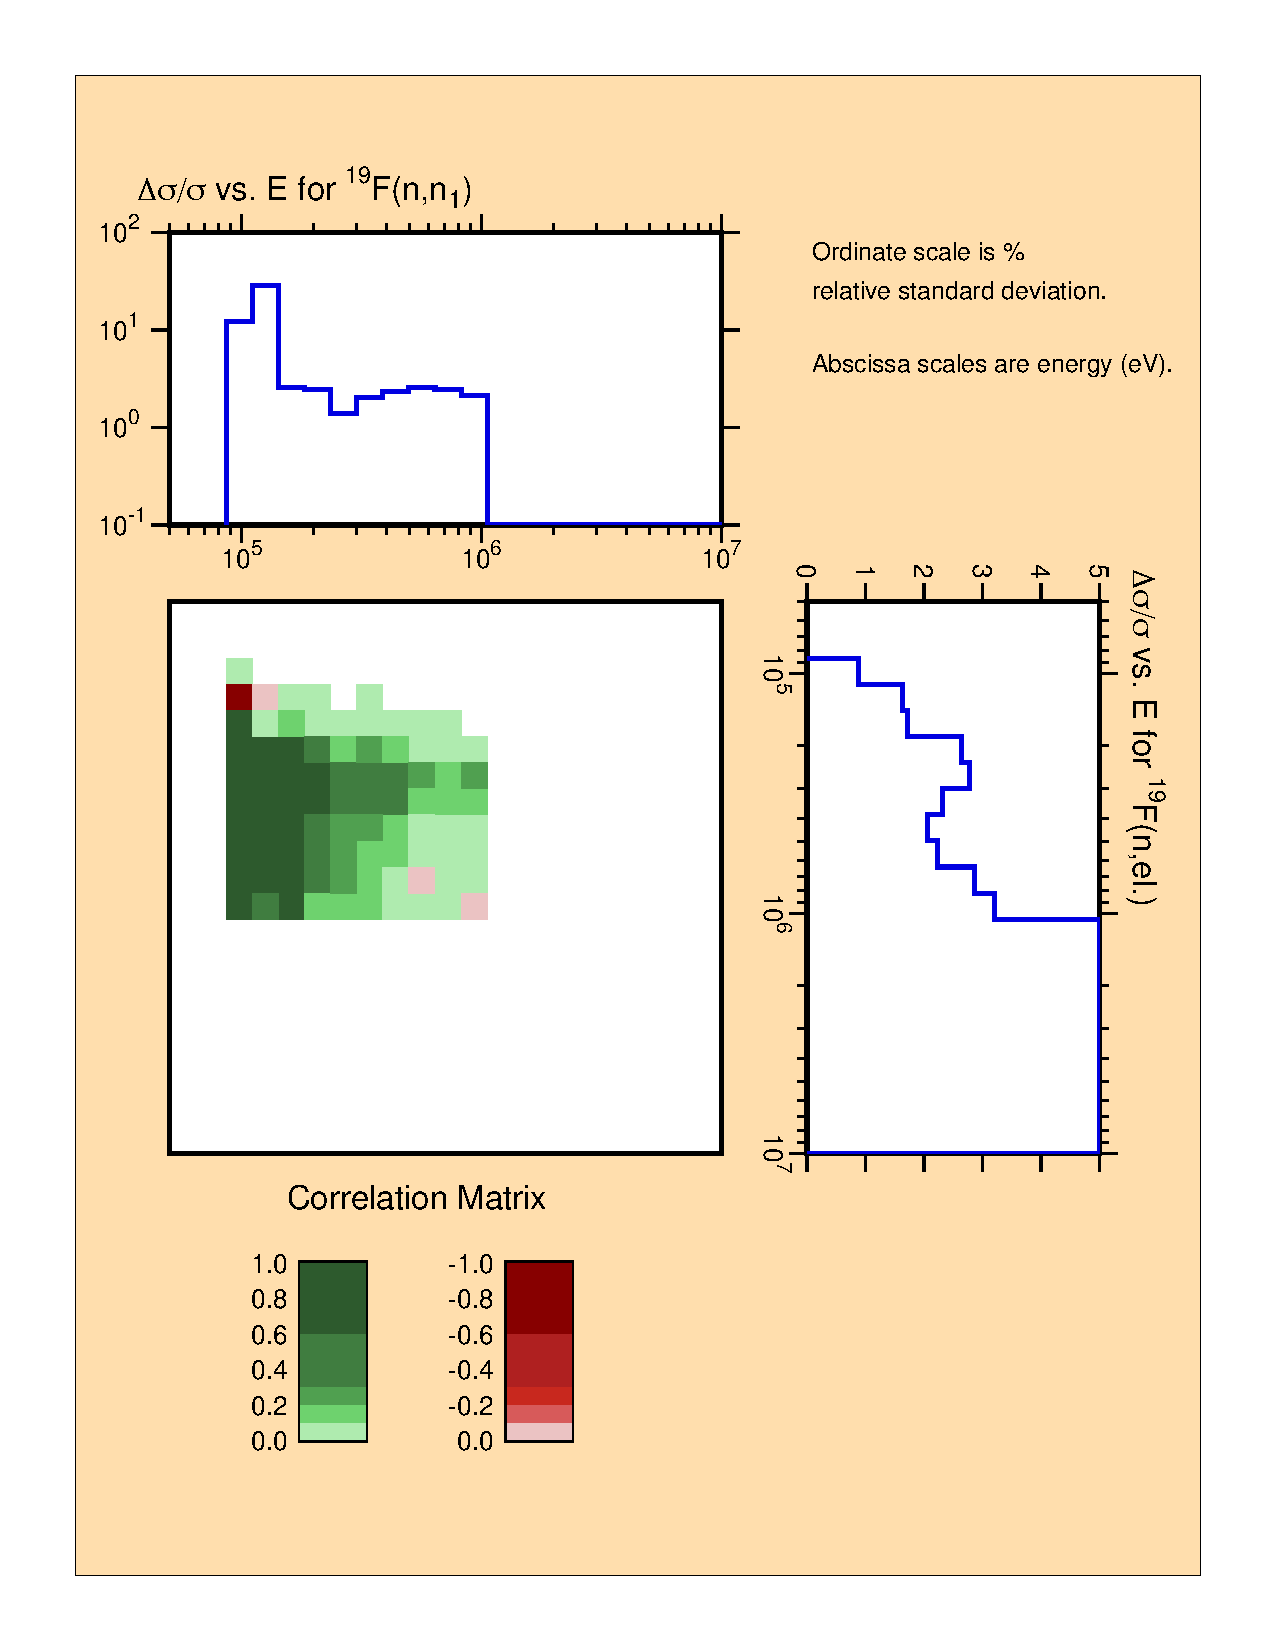
\includegraphics[keepaspectratio, width=5in,angle=0]{figs/covyyack}
\caption[Example of elastic scattering and (n,n$_1$) covariance data]
{Covariance plot for the elastic and (n,n$_1$) reactions from a
 sample ORNL evaluation for $^{19}$F, demonstrating the channel-channel
 covariances possible when using the Reich-Moore-Limited resonance
 representation.}
\label{covyy}
\end{figure}

\subsection{Secondary Particle Angular Distribution Covariances---File 34}
\label{ssERRORR_34}

File 34 contains covariances for angular distributions of secondary
particles.  While the underlying angular distribution data in File 4
may be given as tabulated distributions or as Legendre polynomial
coefficients, File 34's covariance data are only given for Legendre
coefficients.  At present there is no provision to specify covariances
between cross sections from File 3 and angular distributions from
File 4, nor to specify angular distribution covariances between
different materials.  The data format is governed by the \cword{LB}
flag discussed above in Section~\ref{ssERRORR_Str} with LB values
of 0, 1, 2, 5 and 6 allowed.

File 34 in the ENDF file may include covariance data for any MT
reaction defined in File 4, but currently NJOY only processes
the $P_1$ component of MT=2 (elastic scattering).

Fig.~\ref{mf34cov} shows an example of the covariances computed from File 34
for $^{238}$U from JENDL-3.3.  As usual, there are three components to this
plot.  On the right side, we illustrate $\bar{\mu}$ {\it vs} energy, which
dislays the expected forward-peaked characteristic with increasing energy;
on the top is
the uncertainty in $\bar{\mu}$ {\it vs} energy; and in the center is the
correlation matrix.   The ERRORR input for this case will be presented
below.

\begin{figure}[thb]\centering
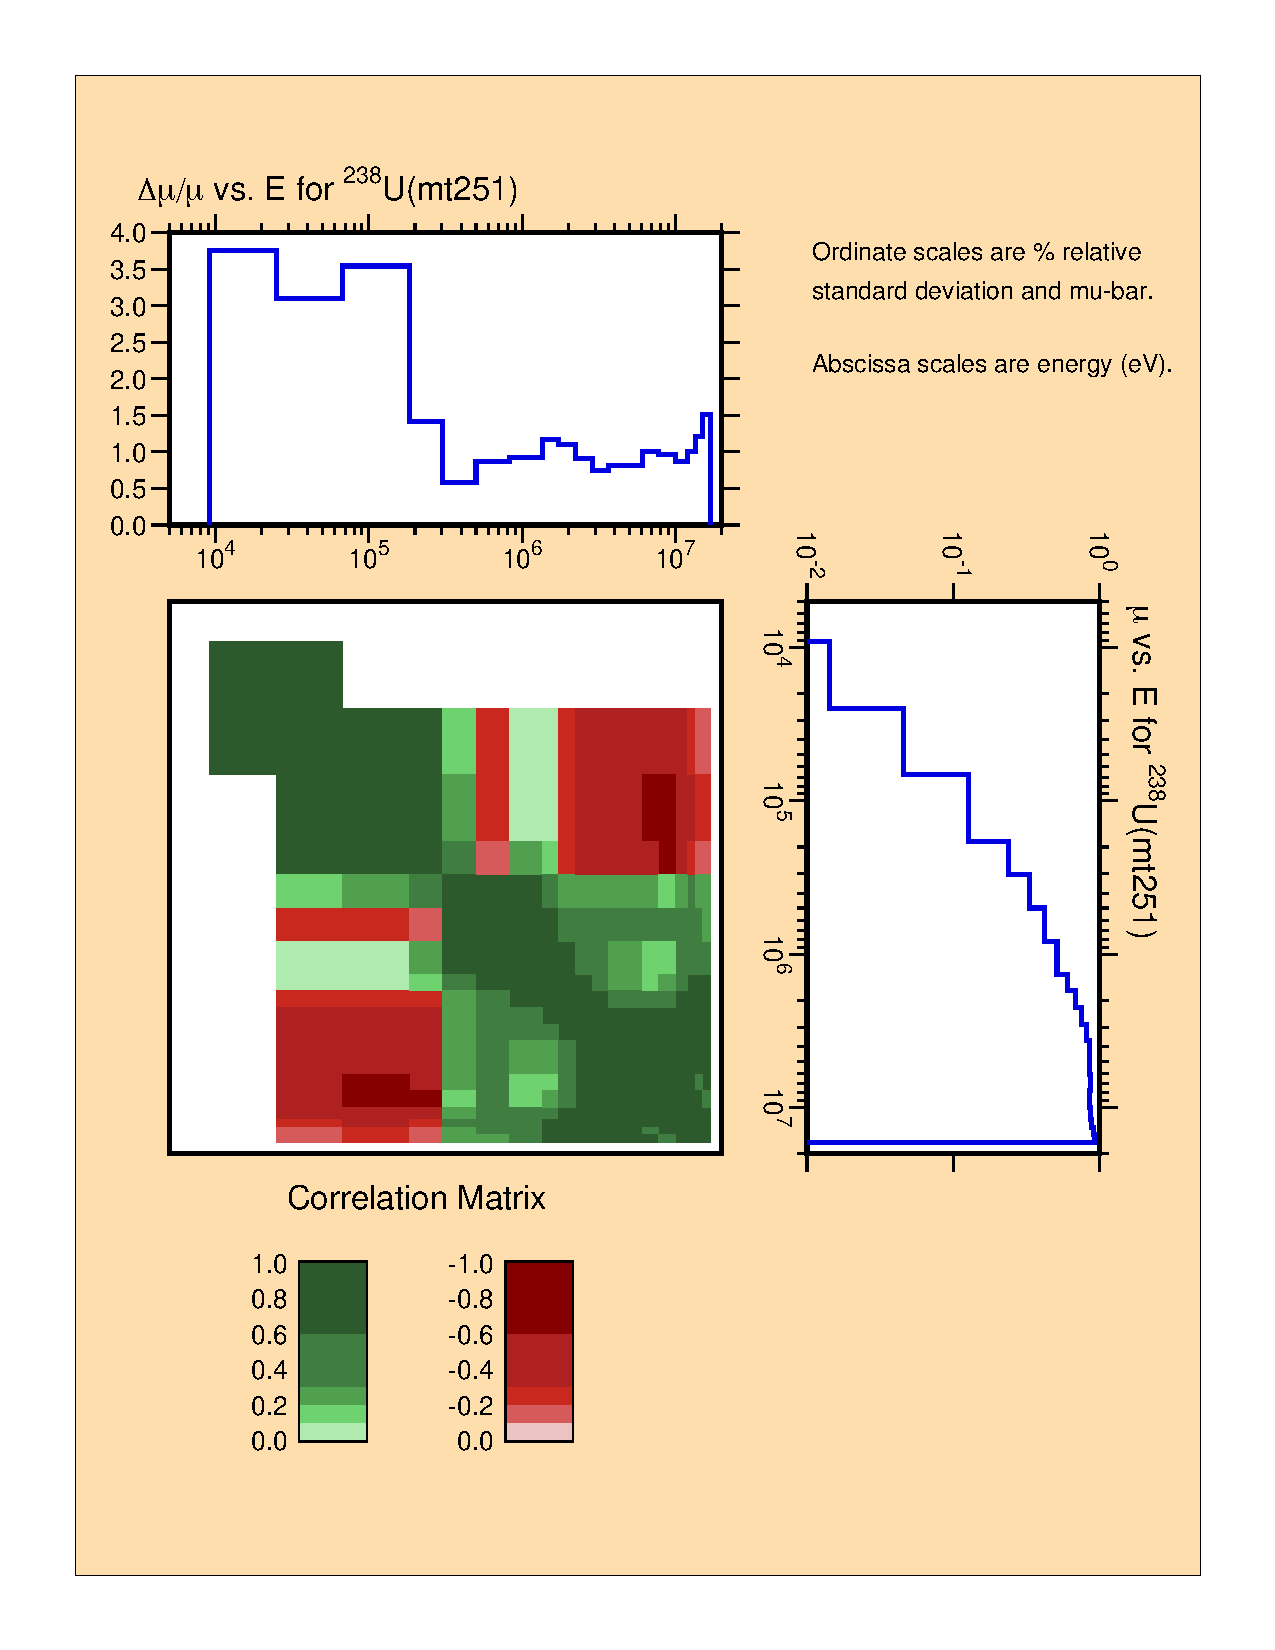
\includegraphics[keepaspectratio, width=5in, angle=0]{figs/mf34covack}
\caption[Example of angular distribution covariance data]{Example of angular
distribution covariance data.}
\label{mf34cov}
\end{figure}

\subsection{Secondary Particle Energy Distribution Covariances---File 35}
\label{ssERRORR_35}

File 35 contains covariance matrices for the energy distributions
of secondary particles given in File 5.  If the spectral distributions
are correlated with angular distributions and given in File 6, the
covariance information still appears in File 35 (the MT section
identifier is the common datum relating these data) and refers
to the angle-integrated distributions only.  The secondary energy
distribution is usually defined on a relatively fine energy grid,
and multiple distributions are given as a function of increasing
incident particle energy.  Since the uncertainties in secondary
distributions are usually highly correlated as a function of incident
particle energy, it is generally sufficient to only define a few
covariance matrices over relatively broad incident energy groups.
There is no provision to specify covariances between these groups
nor with data from other files such as File 3 cross sections or
File 1 prompt, delayed or total $\bar{\nu}$.

File 35 covariance data are given in a series of \cword{NK} subsections,
with each subsection covering a unique incident particle energy range.
The lowest energy of the first subsection and the highest energy of
the last subsection must cover the entire incident particle energy
range from File 5 (or File 6).  When processing MF35 data, the user
can specify the incident particle energy of interest (\cword{efmean}
on Card 7).  NJOY will process the \cword{NK}$^{\rm th}$ subsection whose
energy is closest to, but less than, \cword{efmean}.  The data
tabulated in the ENDF file are normalized probabilities of absolute
covariances identified as an \cword{LB}=7 subsection.  \cword{LB}=7
is identical to \cword{LB}=5 defined in Section~\ref{ssERRORR_Str}
except that these data are now absolute rather than relative covariances.

The ENDF format manual notes these matrices are probability distributions
that must remain normalized to unity and therefore the elements in these
symmetric matrices are constrained such that the sum of the elements
in any row (or column) must be zero.  This is sometimes referred to as
the ``zero sum" rule.  Of course, when dealing with real
numbers of finite precision whose values can vary by orders of magnitude
it is virtually impossible to rigorously conform to this rule.
Therefore, if the sum is sufficiently small, the rule is judged to be
satisfied.  If not, the ENDF manual provides a correction formula
to apply to all matrix elements.  When processing File 35 data NJOY,
checks this summation requirement and, if necessary, applies the
required correction.  NJOY uses the ``sufficiently small" criteria
specified in the Format manual for this check.

At present there are no File 35 data in ENDF/B-VII.0 neutron files,
but the $^{252}$Cf decay file does contain such data.  Also, these data
are becoming available in preliminary ENDF/B-VII.1 files available from
the National Nuclear Data Center (NNDC) at Brookhaven
National Laboratory (BNL).  These files follow
the ``zero sum' rule discussed above, but users are cautioned that
other internationally distributed files, particularly those from
JENDL-3.3, may provide File 35 data in an alternate format.  The
matrix elements in the JENDL-3.3 files have been divided by the
group energy width to yield energy-group averaged probability
distributions, as this is the data representation expected by the
Japanese ERRORJ code\cite{ERRORJ}\index{ERRORJ}.  A conversion code,
chmf35, has been developed and is available from the Nuclear Energy Agency
\footnote{chmf35 may be downloaded from
\href{http://www.nea.fr/dbprog/Njoy/chmf35.for}
{http://www.nea.fr/dbprog/Njoy/chmf35.for}}
to reformat these files
so that they are suitable for processing by NJOY.

Fig.~\ref{mf35cov}
shows the results of processing the ficticious $^{252}$Cf evaluation.  The
ERRORR input for this job will be presented below.

\begin{figure}[thb]\centering
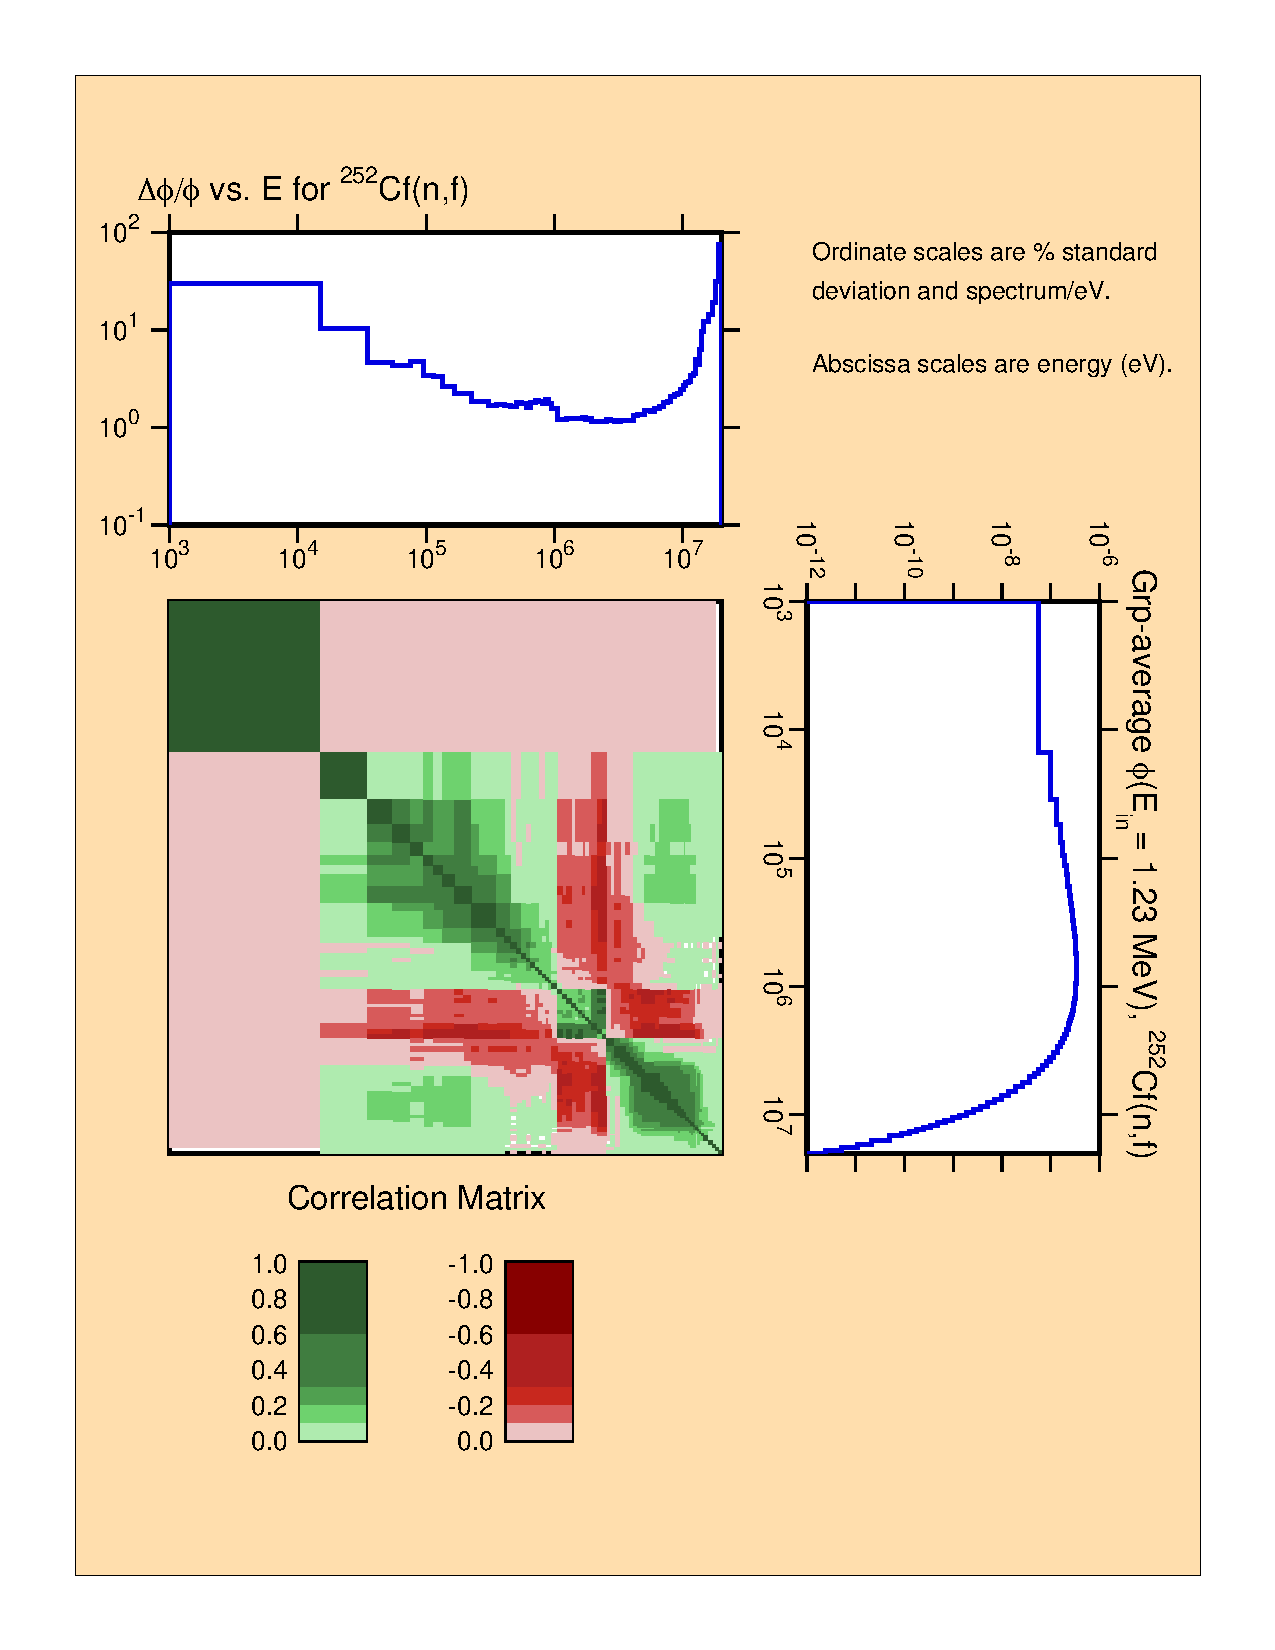
\includegraphics[keepaspectratio, width=5in, angle=0]{figs/mf35covack}
\caption[$^{252}$Cf(n,f) spontaneous fission spectrum covariance data]{Example
 of energy distribution covariances.  The appearance of negative correlations
 results from the requirement for preserving normalization.}
\label{mf35cov}
\end{figure}

\subsection{Radioactive Nuclide Production Covariances--File 40}
\label{ssERRORR_40}

There is only one file in ENDF/B-VII.0 that includes File 40 covariance
data -- $^{93}$Nb.  The input for calculating the $^{93m}$Nb production
uncertainty will be shown below, but the resulting covariances are shown
here in Fig.~\ref{mf40cov}.  The form of the graphical output
obtained when processing File 40 is identical to that produced when
processing File 33; with the cross section shown to the right, the
uncertainty shown to the top and the correlation matrix shown in the
center.  That these are File 40 data can be determined from the label
on the uncertainty portion of the plot.  In 2009, the File 40 format
was modified to include the \cword{IZAP} parameter that identifies the daughter
product.  We include this \cword{IZAP} value in the plot label so that the user
can more fully identify these data.  If an older File 40 file is processed
that does not define \cword{IZAP}, then the text string ``\cword{MF40}'' will
appear in the title.  In the example shown here we have modified the original
ENDF/B-VII.0 $^{93}$Nb file to include the proper \cword{IZAP} value in
File 40, which then appears in the plot title.

\begin{figure}[t]\centering
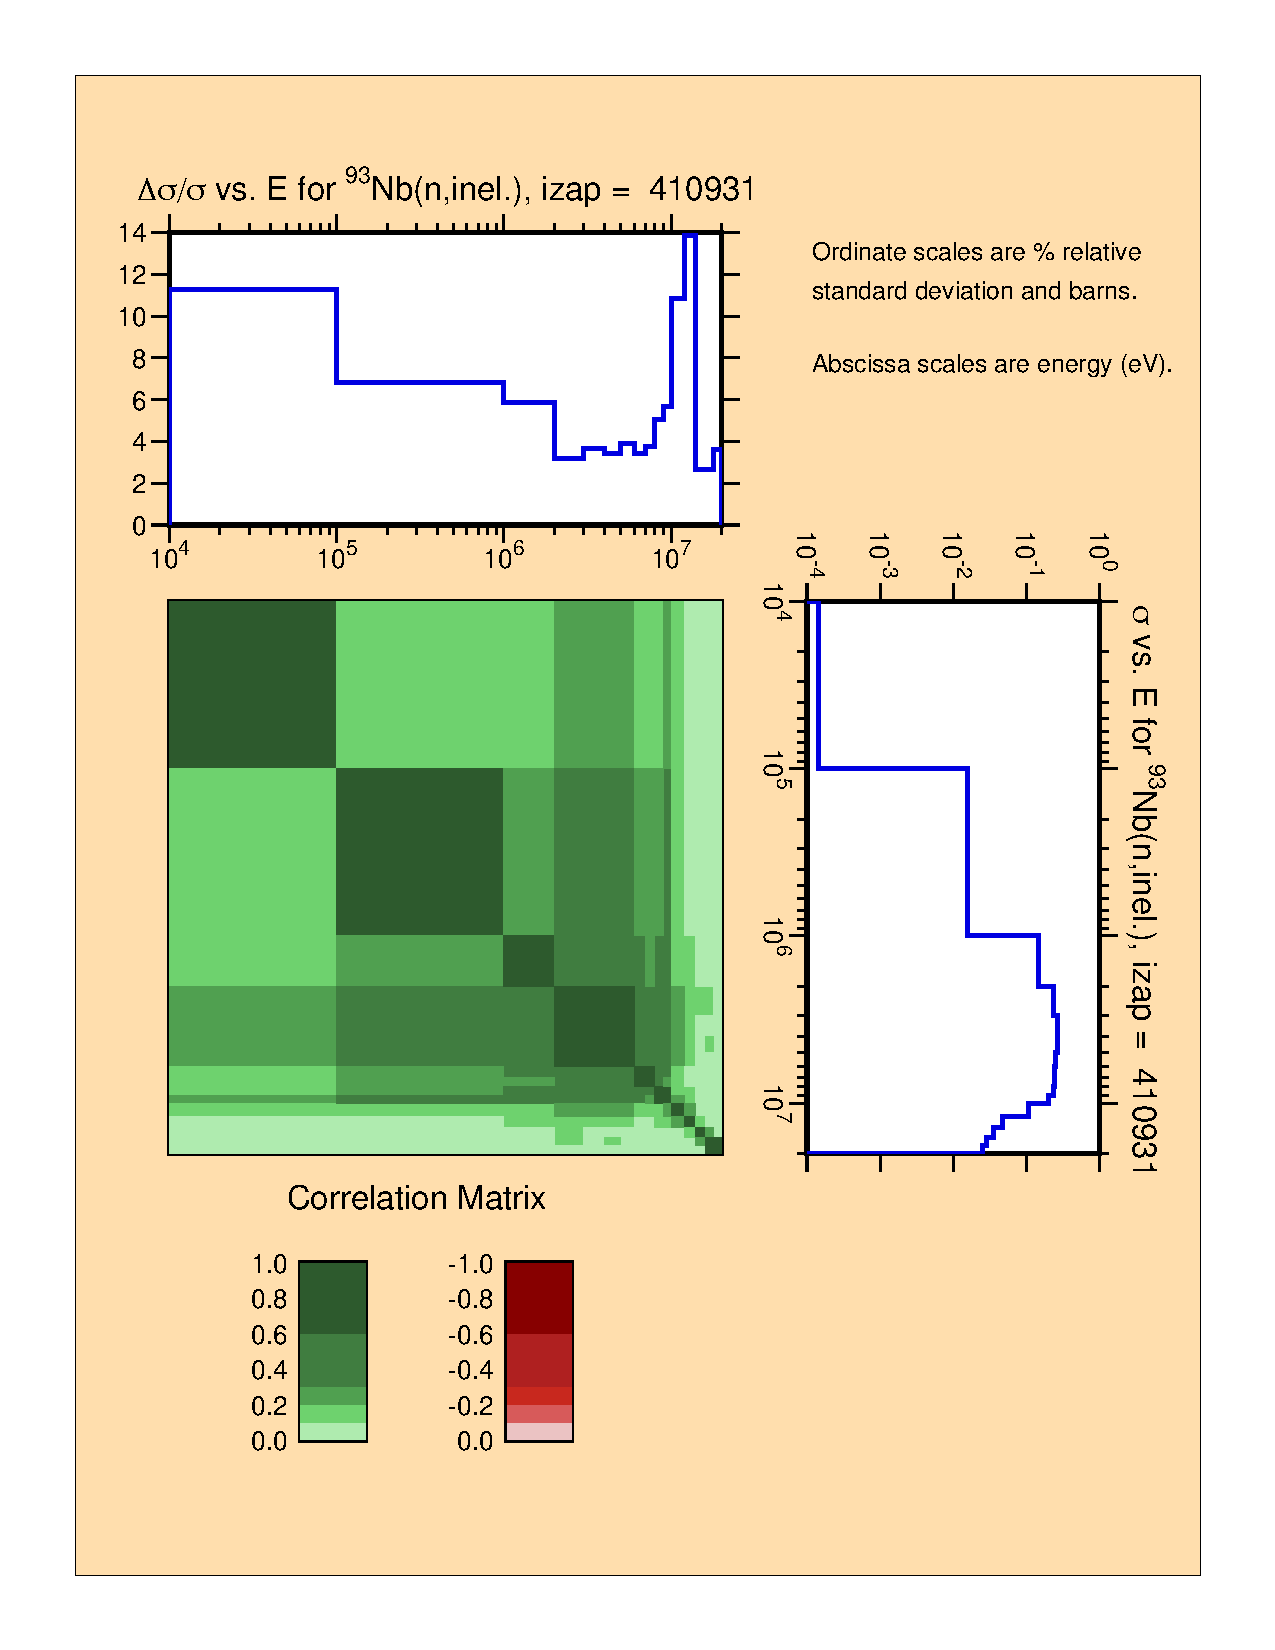
\includegraphics[keepaspectratio, width=5in, angle=0]{figs/mf40covack}
\caption[Radioactive nuclide production covariance example]{Example of
 radioactive nuclide production covariances.}
\label{mf40cov}
\end{figure}

\subsection{Calculation of Multigroup Fluxes, Cross Sections, and
 Covariances on the Union Grid}
\label{ssERRORR_UnionGrid}

As mentioned before, the main function of the ERRORR module is to
calculate the uncertainty in group-averaged cross sections at infinite
dilution due to uncertainty in the ENDF point data.  In this and the
following sections, we describe the procedures used in performing this
task.

In order to proceed, it is necessary to introduce into the discussion
three different energy grids, namely, the user grid, the ENDF grid, and
the union grid.  The relationship of these three grids is shown in
Fig.~\ref{grel}.  The user grid is the multigroup structure in which
the output multigroup covariances are to be produced.  The ENDF grid
is the collection of energies obtained (in subroutines
\cword{gridd}\index{gridd@{\ty gridd}} and
\cword{grist}\index{grist@{\ty grist}}) by forming
the union of (a) all energy ``lists'' appearing in any NI-type
sub-subsection of any subsection to be processed in the current ENDF
material, and (b) all energy pairs used to define the range of
effectiveness of any NC-type sub-subsection of any subsection to be
processed.  The union grid, on the other hand, is simply the union of
the user grid and ENDF grid.  The utility of the union grid is that (a)
the covariances are particularly simple to calculate in this grid, as
discussed below, and (b) the multigroup covariances needed by the user
are then easily obtained by a straightforward collapse from this to
the user grid.  In fact, the design of the current ENDF covariance
format was strongly influenced by the desire to employ this particular
procedure for multigroup processing\cite{Weisbin,Smith}.

\begin{figure}[b]\centering
$\begin{array}{lccccccccr}
{\rm User\; Grid} \; \;  &|&& \phi_1 , X_1  &  &|& & \phi_2 , X_2   &   &| \\
{\rm ENDF\; Grid} \; \;  &|& F_1 \; &|& &  F_2 & & |&  F_3               &| \\
{\rm Union \;Grid}  \; \;  &|&\phi_1 , x_1 &|& \phi_2 , x_1 &|&\phi_3 ,
   x_3 & | &\phi_4, x_4 &|\\
\end{array}$
\vspace{.25 in}
\caption{Illustration of energy grid relations.}
\label{grel}
\end{figure}

After the union grid is formed in subroutine
\cword{uniong}\index{uniong@{\ty uniong}}, the cross
sections $x(E)$ and weighting flux $\phi (E)$ are integrated to produce
$x_I$ and $\phi_I$, multigrouped on this grid.  If point cross sections
are supplied, an exact integration is done in subroutine
\cword{grpav}\index{grpav@{\ty grpav}}.  If, on the other hand, a
multigroup cross-section library is supplied, then subroutine
\cword{colaps}\index{colaps@{\ty colaps}} is used.  If a library group
is subdivided by a union-group boundary, then over the span of that
library group, the unknown energy dependencies of $x(E)$ and $\phi
(E)$, which are needed to calculate $x_I$ and $\phi_I $, are
approximated in subroutine \cword{colaps} by constants.  Normally, the
effect of this approximation is not large and, in any case, can be
reduced or eliminated by increasing the number of groups in the input
library.

We next consider the theoretical basis for the calculation of
union-grid multigroup covariances, as performed in subroutine
\cword{covcal}\index{covcal@{\ty covcal}}.  By definition, $x_I$
is just the average of $x(E)$ over union group I,

\begin{equation}
   x_I \; \equiv \;\frac  {\displaystyle\int_I \; \phi (E) \; x(E) \;
  dE}{\displaystyle\int_I \; \phi (E) \; dE} \,\,,
\label{e19}
\end{equation}

\noindent
where $\phi (E)$ is the flux ``model'' assumed for the multigroup
calculations.  Let $y_J$ denote similarly the average of $y(E)$ over
union group $J$.

Let us imagine that these groups are subdivided into many subintervals
of infinitesimal width, so that in the i$^{\rm{th}}$ subinterval of group I,
for example, $x(E)$ can be well approximated by the constant $x_i$.  By
this device, the integrals that define $x_I$ and $y_J$ can be converted
to discrete sums:

\begin{equation}
x_I \; = \frac{{\displaystyle \sum_{i\in I}} \; \phi_i \; x_i}{\phi_I } \; = \;
\sum_{i\in I} \; \alpha_{Ii} \; x_i\,\,,
\label{e20}
\end{equation}

\noindent
where

\begin{eqnarray}
\phi_i & = & \int_{i} \; \phi (E) \; dE \;,\\
\nonumber \\
\phi_I & = & \sum_{i\in I} \; \phi_{i} \; = \; \int_{I} \; \phi (E) \; dE\;,
\end{eqnarray}

\noindent
and

\begin{equation}
\alpha_{Ii} \equiv \frac{\phi_i}{\phi_I} \; .
\end{equation}

\noindent
From these definitions, clearly

\begin {equation}
\sum_{i\in I}\; \alpha_{Ii} \; = \; 1 \; .
\label{e24}
\end{equation}

\noindent
Similarly for $y$,

\begin{equation}
y_J = \sum_{j\in J} \; \alpha_{Jj} \; y_j\;,
\label{e25}
\end{equation}

\noindent
and

\begin{equation}
\sum_{j \in J} \; \alpha_{Jj} = 1 \;.
\label{e26}
\end{equation}

The methodology of ERRORR assumes that $\phi(E)$ in Eq.~\ref{e19} is
free of uncertainty.  Under this assumption, the terms $\alpha_{Ii}$
and $\alpha_{Jj}$ are simply known constants.  The covariance of $x_I$
with $y_J$ can then be calculated using the propagation-of-errors
formula, Eq.~\ref{e11}, together with Eqs.~\ref{e20} and \ref{e25}.

\begin{eqnarray}
{\rm {\rm cov}} (x_I,y_J) & = & \sum_{i\in I\atop{j\in J}}\;
  \alpha_{Ii} \; \alpha_{Jj} \; {\rm cov}
 (x_i ,y_j) \nonumber \\
\nonumber \\
 & = & \sum_{i\in I\atop{j\in J}}\; \alpha_{Ii} \; \alpha_{Jj} \; \sum_{n}{\rm
 cov} (x_i ,y_j)_n \; ,
\end{eqnarray}

\noindent
where the summation over $n$ results from the different independent
contributions to the ENDF point covariances coming from the different
NI-type sub-subsections.  Changing the order of summation, we obtain

\begin{equation}
{\rm  cov} (x_I,y_J) \; = \; \sum_{n} \; {\rm cov} (x_I,y_J)_n \; ,
\label{e28}
\end{equation}

\noindent
where
\begin{equation}
{\rm cov} (x_I,y_J)_n \;=\; \sum_{i\in I\atop{j\in J}} \; \alpha_{Ii}\;
\alpha_{Jj}\;\; {\rm {\rm cov}} (x_i,y_j)_n \; .
\label{e29}
\end{equation}

To evaluate the sum in Eq.~\ref{e29}, we make use of the fact that union
groups {\it I} and {\it J} do not cross any ENDF grid boundaries.
Recalling the discussion of NI-type sub-subsections (and
excluding for the moment the case where sub-subsections with
\cword{LB}=8 are present), there are only two possibilities for the
energy dependence of the covariance between ENDF grid points; thus,
over the limits of the sum, either cov$(x_i,y_j)_n$ is independent of
$i$ and $j$ (if \cword{LB}=0) or rcov$(x_i,y_j)_n$ is independent of
$i$ and $j$ (if $1\leq$ \cword{LB} $\leq 6$).  We consider first the
constant-absolute-covariance case, \cword{LB}=0.  Eq.~\ref{e29} can then be
rewritten as follows:

\begin{equation} {\rm {\rm cov}} (x_I,y_J)_n\; = \; {\rm {\rm cov}} (x,y)_n
\; \sum_{i\in I\atop{j\in J}} \; \alpha_{Ii} \; \alpha_{Jj} \; = \;
  {\rm {\rm cov}} (x,y)_n
\left(\sum_{i\in I} \; \alpha_{Ii} \right) \left(\sum_{j\in J} \;
  \alpha_{Jj}\right) \; .
\end{equation}

\noindent
Invoking Eqs.~\ref{e24} and \ref{e26}, we obtain

\begin{equation}
{\rm cov}(x_I , y_J)_n \;=\; {\rm cov}(x,y)_n \; \;\;\;\;\;
  (\hbox{\cword{LB}} = 0) \;.
\label{e31}
\end{equation}

\noindent
For \cword{LB}-values ranging from 1 to 6, the relative covariance is
constant over each union group, so we rewrite Eq.~\ref{e29} in the form

\begin{eqnarray}
{\rm {\rm cov}} (x_I,y_J)_n & = & \sum_{i\in I\atop{j\in J}}\; \alpha_{Ii}\;
  \alpha_{Jj} \; x_i \; x_j \;
{\rm r{\rm cov}} (x_i , x_j)_n \nonumber \\
  & = &{\rm r{\rm cov}} (x,y)_n \sum_{i\in I\atop{j\in J}}\;
 (\alpha_{Ii}\; x_i ) \; (\alpha_{Jj} \; y_j) \nonumber \\
  & = & {\rm rcov} (x,y)_n \; \left(\sum_{i\in I} \; \alpha_{Ii} \;
  x_i \right) \left(\sum_{j\in J}\; \alpha_{Jj} \; y_j \right) \; .
\label{e32}
\end{eqnarray}

\noindent
Substituting here from Eqs.~\ref{e20} and \ref{e25}, we obtain

\begin{equation}
{\rm {\rm cov}} (x_I , y_J)_n = x_I\; y_J \; {\rm r{\rm cov}} (x,y)_n
  \;\;\;\;\;\; (1
\leq\hbox{\cword{LB}}\leq 6)\; .
\label{e33}
\end{equation}

\noindent
The final union-group multigroup covariance is obtained by inserting
these results, Eqs.~\ref{e31} and \ref{e33}, back into Eq.~\ref{e28}

\begin{equation} {\rm cov} (x_I,y_J) = \; \sum_{\rm n(LB=0)}  \;
{\rm cov} (x,y)_n \;+\; \sum_{\rm  n(LB=1,6)}  \;x_I\;y_J
\; {\rm r{\rm cov}} (x,y)_n\;,
\label{e34}
\end{equation}
\vspace{1 pt}

\noindent
where the first sum runs over all sub-subsections with \cword{LB}=0 and
the second runs over all sub-subsections with \cword{LB}=1 through 6.  The
quantities cov$(x,y)_n$ and r{\rm cov}$(x,y)_n$ here
are simply the point-energy covariances from the ENDF covariance file,
as described in Eqs.~\ref{e12} through \ref{lbopts}.  Equation \ref{e34}
then is the basic equation used in subroutine \cword{covcal} to
calculate the desired union-group covariances.

The final step, if sub-subsections with \cword{LB}=8 are present, is to
increment the diagonal elements (variances) as follows:

\begin{equation}
{\rm cov} (x_I, x_I) = {\rm cov} (x_I, x_I) +
F_k\,(E_{k+1} - E_k)/\Delta E_I \;,
\label{e35}
\end{equation}

\noindent
where k indexes the range of the \cword{LB}=8 energy grid that includes
union group {\it I}.

\subsection{Basic Strategy for Collapse to the User Grid}
\label{ssERRORR_GridStrategy}

The union-group fluxes $\phi_I$ are used, in subroutine
\cword{sigc}\index{sigc@{\ty sigc}}, to collapse the union-group
cross sections to the coarser user grid.  Changing notation slightly,
let us denote by $x_I(a)$ the cross section in union group {\it I}
for reaction $a$, and similarly let $X_K (a)$ be the cross section
in user group {\it K} for the same reaction.  In complete analogy
with Eq.~\ref{e20},

\begin{equation}
X_K(a) = \frac {\displaystyle{\sum_{I\in K}\; \phi_I\;x_I(a)}}{\phi_K}
 \;=\; \sum_{I\in K} \; A_{KI} \; x_I(a)\;,
\end{equation}

\noindent
where

\begin{equation}
\phi_K = \sum_{I\in K} \;\phi_I \;,
\end{equation}

\noindent
and

\begin{equation}
A_{KI} = \frac{\phi_I}{\phi_K}\;.
\end{equation}

\noindent
Applying the propagation-of-errors formula again gives

\begin{equation}
{\rm cov} \left[X_K(a),X_L(b) \right] = \sum_{I\in K\atop{J\in L}}\;
  A_{KI}\;A_{LJ}\;{\rm {\rm cov}}[x_I(a),x_J(b)] \;.
\label{e39}
\end{equation}

\noindent
An alternative expression, obtained by simply rearranging coefficients, is

\begin{equation}
{\rm {\rm cov}} \left[X_K(a),X_L(b) \right] =
  \frac{1}{\phi_K \phi_L} \sum_{I\in K\atop{J\in L}} \; T_{IJ}(a,b) \; ,
\label{e40}
\end{equation}

\noindent
where

\begin{equation}
T_{IJ}(a,b) = \phi_I\;\phi_J \; {\rm cov} [x_I(a),x_J(b)]\;.
\label{e41}
\end{equation}
\vspace{1 pt}

\noindent
Eqs.~\ref{e40} and \ref{e41} provide the basic framework in the ERRORR
module for the production of multigroup covariances in the coarse user-group
structure.  Finally, if requested, the Eq.~\ref{e40} absolute covariances
are converted to relative form,

\begin{equation}
{\rm r{\rm cov}} [X_K(a),X_L(b)] =
  \frac{{\rm cov} [X_K(a),X_L(b)]}{X_K(a)\;X_L(b)} \;.
\label{e42}
\end{equation}

\subsection{Group-Collapse Strategy for Data Derived by Summation}
\label{ssERRORR_summ}

The procedure described in the previous section must be modified if, in
some energy range, either reaction $a$ or $b$ is a ``derived'' quantity
in the sense of Eq.~\ref{e17} or Eq.~\ref{e18}.  In such a case, one
cannot apply Eq.~\ref{e34} directly to the calculation of
${\rm {\rm cov}}[x_I (a),x_J(b)]$, because the covariances on the
right-hand side of Eq.~\ref{e34} will be missing from the ENDF file in
the affected energy region.

We consider first the case in which some cross sections are evaluated
(``derived'') by simply summing other evaluated cross sections, as in
Eq.~\ref{e17}.  Equation \ref{e35} can then be rewritten as

\begin{equation}
X_K(a) = \sum_{I\in K} \; A_{KI} \;\left\{\sum_{{\rm all\; c}} \;
  C_I(a,c)\;x_I(c)\right\} \;,
\end{equation}

\noindent
where the quantity in curly brackets is the value of the derived cross
section ``a'' in union group {\it I}, as reconstructed from the
directly evaluated cross sections $x_I (c)$.  The derivation
coefficients $C_I (a,c)$ depend on the union-group index {\it I},
because the evaluator is permitted to employ different derivation
strategies in different energy ranges in order to simplify and shorten
the covariance files.

To expand on this last point, suppose there are only three reactions,
and suppose that the cross sections $x(1)$ and $x(2)$ rigorously sum to
$x(3)$ at all energies.  Further suppose that within the
energy range {\rm cov}ered by the first union group, the cross-section
evaluator has used this logical connection in order to ``derive''
$x(3)$, that is to evaluate $x(3)$, by summing the existing evaluations
for $x(1)$ and $x(2)$,

\begin{equation}
x_1(3) = x_1(1)\;+\;x_1(2)\;.
\end{equation}

\noindent
Further suppose that in the range of union group 2, $x(1)$ is derived by
employing the same logical connection, but in a different way,

\begin{equation}
x_2(1) = x_2(3)-x_2(2)\;,
\end{equation}

\noindent
and in union group 3, all three reactions are directly evaluated.

In this example $C_I(a,c)$ has the following values:
\begin{center}
$\begin{array}{lll}

\makebox[1.25in]{
$\begin{array}{llr}
C_1(1,1) & = & 1 \\
C_1(2,1) & = & 0\\
C_1(3,1) & = & 1
\end{array}$}
&
\makebox[1.25in][l]{
$\begin{array}{llr}
C_1(1,2) & = & 0 \\
C_1(2,2) & = & 1 \\
C_1(3,2) & = & 1
\end{array}$}
&
\framebox[1.25in]{
$\begin{array}{llr}
C_1(1,3) & = & 0 \\
C_1(2,3) &= & 0 \\
C_1(3,3) & = & 0
\end{array}$}
\\
\\
\framebox[1.25in]{
$\begin{array}{llr}
C_2(1,1) & = & 0 \\
C_2(2,1) & = & 0 \\
C_2(3,1) & = & 0 \\
\end{array}$}
&
\makebox[1.25in][l]{
$\begin{array}{llr}
C_2(1,2) & = & -1 \\
C_2(2,2) & = & 1 \\
C_2(3,2) & = & 0
\end{array}$}
&
\makebox[1.25in]{
$\begin{array}{llr}
C_2(1,3) & = & 1 \\
C_2(2,3) & = & 0 \\
C_3(3,3) & = & 1
\end{array}$}
\\
\\
\makebox[1.25in]{
$\begin{array}{llr}
C_3(1,1) & = & 1 \\
C_3(2,1) & = & 0 \\
C_3(3,1) & = & 0
\end{array}$}
&
\makebox[1.25in][l]{
$\begin{array}{llr}
C_3(1,2) & = & 0 \\
C_3(2,2) & = & 1 \\
C_3(3,2) & = & 0
\end{array}$}
&
\makebox[1.25in]{
$\begin{array}{llr}
C_3(1,3) & = & 0 \\
C_3(2,3) & = & 0 \\
C_3(3,3) & = & 1
\end{array}$}
\end{array}$
\end{center}

\noindent
Note that in all cases we have formally considered the evaluated cross
sections to be derived from themselves, $C_I(a,c)|_{\rm eval}{=}
\delta_{ac}$.  This device allows us to use Eq.~\ref{e42} for all
reactions, regardless of whether they are derived or
evaluated.  Note that, in every case where reaction $c$ is
derived in group $I,\; C_I(a,c) {=} 0$.  (See boxed submatrices.)
This null ``sensitivity coefficient'' is important, because it means
that Eq.~\ref{e42} remains a linear relation involving only dependent
quantities with known covariances (the evaluated subset
of the union-group cross sections) on the right.  This allows us once
again to use the propagation-of-errors formula to obtain the desired
user-group covariances.

\begin{equation}
{\rm cov} [X_K,(a),X_L(b)] = \sum_{{\rm all \; c\;} \atop{\rm all \;d\;}}
 \sum_{I\in K\atop {J \in L}} \; A_{KI} \; C_I (a,c) \; A_{LJ} \;
   C_J (b,d) \; {\rm {\rm cov}} [x_I(c),x_J(d)]\; ,
\label{e46}
\end{equation}

\noindent
or, alternatively,

\begin{equation}
{\rm {\rm cov}} [X_K,(a),X_L(b)] = \frac{1}{\phi_K \phi_L}\;
  \sum_{{\rm all \; c\;} \atop{\rm all \;d\;}}
 \sum_{I\in K\atop {J \in L}} \; C_I(a,c)\; C_J(b,d) \; T_{IJ}(c,d)\; ,
\end{equation}

\noindent
where
\begin{equation}
T_{IJ}(c,d) = \phi_I\; \phi_J \; {\rm {\rm cov}} [x_I(c),x_J(d) ] \; .
\end{equation}

In subroutine \cword{covcal}\index{covcal@{\ty covcal}}, the
flux-covariance product $T_{IJ}$ is calculated for all evaluated
reaction pairs and written to a ``scratch'' binary disk file, unit 11.
 (For diagnostic purposes, it is possible to change this to a
formatted scratch file by manually resetting the variable
\cword{imode} to  $+1$ in the main program.)  In
the subsequent collapse to the user's group structure in
subroutine \cword{covout}, the user-group covariances ${\rm {\rm
cov}}[X_K(a),X_L(b)]$ for one specific a-b reaction pair, for all
``\cword{MT1}'' energy groups L, and for as large a range of ``\cword{MT}''
energy groups K as possible, are calculated simultaneously in memory.

In \cword{covout}\index{covout@{\ty covout}}, the disk file (unit 11)
is rewound and read completely through, once in each range of MT groups
for each a-b reaction pair, to access the union-group covariances for
the evaluated reactions.  As the union-group data pass through memory,
contributions to the user-group covariances are accumulated using
Eq.~\ref{e46}.

In the fairly common situation where cross sections $x(a)$ and $x(b)$
are directly evaluated over the whole energy range of the data
file,

\begin{equation}
C_I(a,c) = \delta_{ac},\; {\rm for \; all} \; I,
\end{equation}

\noindent
and

\begin{equation}
C_J(b,d) = \delta_{bd},\; {\rm for \; all} \; J.
\end{equation}

\noindent
In this case, Eq.~\ref{e46} can be greatly simplified.

\begin{eqnarray}
  {\rm {\rm cov}} [X_K(a),X_L(b)] & =
  & \frac{1}{\phi_K \phi_L}\;\sum_{{\rm all \; c\;}
  \atop{\rm all \;d\;}}
  \sum_{I\in K\atop {J \in L}} \;\delta_{ac} \; \delta_{bd} \;
  T_{IJ} (c,d)  \nonumber \\ & = &
  \frac{1}{\phi_K \phi_L} \sum_{I\in K\atop {J \in L}} \;
  T_{IJ} (a,b) \; .
\end{eqnarray}

This result, which is identical to Eq.~\ref{e39}, suggests a shortcut
calculational path, which is followed in subroutine
\cword{covout}\index{covout@{\ty covout}} whenever both reactions
are directly evaluated.  In preparation for this situation, a second
copy of the \cword{covcal}\index{covcal@{\ty covcal}} binary output file
is generated when \cword{covout} is first called.  The second copy, on
unit 12, is read only in the trivial derivation cases just described
(flagged in the code by setting \cword{isd}=1).  Unit 12 is not rewound
before processing a given reaction pair a-b, since earlier reaction
pairs on the file do not contribute to the sum in Eq.~\ref{e46} in these
cases.  Reading of the second copy stops after the union-group
covariances for reaction pair a-b are found, because the later reaction
pairs do not contribute either.


\subsection{Processing of Data Derived from Ratio Measurements}
\label{ssERRORR_Ratio}

The treatment of implicit covariances that arise from ratio
measurements, as in Eq.~\ref{e18}, is totally different from the treatment
of data derived by summation, Eq.~\ref{e17}, discussed in the previous
section.  Before discussing the processing details, it is helpful first
to review the subject of ratio evaluations generally.  Returning to the
``x-y'' notation of Section~\ref{ssERRORR_Defs}, let $x(E_x)$ be the
value of the cross
section for reaction $x$ at energy $E_x$, and $y(E_y)$ the cross
section for reaction $y$ at energy $E_y$.  In some energy region
$(L_x,H_x)$, suppose that the best knowledge of $x(E_x)$ is obtained
through the application of a measured ratio, $u(E_x)$:

\begin{equation}
x(E_x) = u(E_x) \; z(E_x), \;{\rm if} \; L_x \leq E_x \leq H_x \; ,
\end{equation}

\noindent
where reaction $z$ is some well-known cross section,
possibly one of the official ENDF/B standard cross sections.
Similarly, suppose $y$ is derived from the same standard, over a
possibly different energy range:

\begin{equation}
y(E_y) = v(E_y) \; z(E_y), \;{\rm if} \; L_y \leq E_y \leq H_y \; .
\end{equation}

\noindent
By performing a first-order Taylor-series expansion and then applying
the formula for propagation of errors, one can obtain an expression for the
contribution to the relative covariance, ${\rm r{\rm
cov}}[x(E_x),y(E_y)],$ that is attributable to these ratio measurements.
In the usual case, where the ratios $u$ and $v$ are only weakly
correlated with the standard cross section $z$, the result is quite
simple:

\begin{equation}
{\rm rcov}[x(E_x),y(E_y)]_{{\rm ratio}} = {\rm rcov}[u(E_x),v(E_y)] +
 {\rm rcov}[z(E_x),z(E_y)]
\end{equation}

\noindent
if $L_x \leq E_x \leq H_x$ and $L_y \leq E_y \leq H_y$, and

\begin{equation}
{\rm rcov} [x(E_x), y(E_y)]_{\rm ratio}= 0 \;\;{\rm otherwise}.
\label{e55}
\end{equation}

\noindent
Thus, in this fairly common evaluation situation, the covariance
separates naturally into a part involving only the measured ratios and
a part involving only the standard.  Because the second contribution,
cov(MT$_z$, MT$_z$), can be read directly from the NI-type
sub-subsections in evaluation for the standard, it is not included
explicitly in the ENDF subsections for the derived quantities,
cov(MT$_x$, MT$_x$) or cov(MT$_y$, MT$_y$).  Instead, the existence of
this additional contribution to the covariance is signalled by the
presence of an NC-type sub-subsection.

The strategy adopted for processing this information in
subroutine \cword{stand}\index{stand@{\ty stand}} is to load the
NI-type sub-subsections from the evaluation of the standard into
the same storage array that is used to store NI-type covariances
from the evaluation for reaction $x$.  From that point on, the data
from the standard are handled just as if they had come from the
evaluation for $x$, but with one exception.  As indicated by
Eq.~\ref{e55}, the covariance contribution
${\rm {\rm cov}}[z(E_x),z(E_y)]$ is \underline{not} added into
the total covariance matrix for the current reaction pair if
either $E_x$ or $E_y$ lies outside the corresponding energy
``window'' $(L_x,H_x)$ or $(L_y,H_y)$, respectively.

As discussed in Section~\ref{ssERRORR_Str}, in addition to identifying
the standard reaction, the NC-type sub-subsection contains a control parameter
\cword{LTY} and two energies \cword{EL} and \cword{EH} whose
significance depends on \cword{LTY}.   ~\cword{LTY} is used to identify
particular evaluation scenarios: reaction $x$ is the same as reaction
$y$ (or at least they are derived from $z$ over the same energy range)
(\cword{LTY}=1); $y$ is identical to the standard (\cword{LTY}=2); or
$x$ is identical to the standard (\cword{LTY}=3).  A fourth
possibility, namely, that $x$, $y$, and $z$ are entirely distinct,
cannot presently be treated with a single NC-type sub-subsection; that
is, there is no \cword{LTY} value defined for this case.  However, as
discussed later, it is still possible to process covariances for this
situation by combining information from sub-subsections in two
different evaluations.  For convenience, we shall refer to this fourth
case as \cword{LTY}=4.

The interrelationship of \cword{LTY}, \cword{EL}, \cword{EH}, and the
windows $(L_x,H_x)$ and $(L_y,H_y)$ used in ERRORR for the
``zeroing-out'' operation of Eq.~\ref{e55}, is summarized below:

\small
\begin{eqnarray}
\mathtt{LTY=1}  \nonumber \\
   &   & (L_x, H_x) = (L_y, H_y) = (\mathtt{EL},\mathtt{EH}) \nonumber \\
\mathtt{LTY=2} \nonumber \\
   &   & (L_x, H_x) =  (\mathtt{EL},\mathtt{EH}) \nonumber \\
   &   & (L_y, H_y) = (10^{-5} \;{\rm eV},\; 20 \;{\rm MeV}) \nonumber \\
\mathtt{LTY=3} \nonumber \\
   &   & (L_x, H_x) = (10^{-5}\; {\rm eV},\; 20 \; {\rm MeV}) \nonumber \\
   &   & (L_y, H_y) =  (\mathtt{EL},\mathtt{EH}) \nonumber \\
\mathtt{LTY=4} \nonumber \\
   &   & (L_x, H_x) =  (\mathtt{EL},\mathtt{EH}) \nonumber \\
   &   & (L_y, H_y) =  (\mathtt{EL'},\mathtt{EH'}) \; .
\end{eqnarray}
\normalsize

\noindent
If the user requests covariance data, ${\rm {\rm cov}}(x,y)$, where $x$
and $y$ are different and both are distinct from the standard
(\cword{LTY}=4), the ERRORR module obtains (\cword{EL,EH}) from the
\cword{LTY}=2 subsection in the evaluation for $x$ that ``points'' to
$z$.  Then, the covariance file for $z$ is read to obtain both (a) the
explicit covariances ${\rm {\rm cov}}(z,z)$ and (b) the second energy
window (\cword{EL}$'$, \cword{EH}$'$), the latter being found in the
\cword{LTY}=3 sub-subsection that points back to $y$.

We will illustrate ratio covariance processing using data from ENDF/B-V.
Table~\ref{ratios} lists all ENDF/B-V reactions that contain ratio-to-standard
covariance data.  The symbols entered in the reaction-by-reaction
matrix indicate which reactions are referenced as standards ($\ast$),
and which reaction pairs have implicit nonzero covariances
(\cword{LTY}).  ERRORR will produce multigroup covariances for any of
the reaction pairs in Table~\ref{ratios} that are marked with ($\ast$) or
(\cword{LTY}).  The cross-material covariances (\cword{LTY}=2, 3, or 4)
must be requested individually using the
\cword{IREAD}=2 option (see Section~\ref{ssERRORR_inp}, especially
the discussion of
Cards 10 and 11).  An attempt to process covariances for any of the
cases \cword{LTY}=1 through 4 without supplying a separate ENDF
tape containing the needed standard will result in an error stop in
subroutine \cword{gridd}.  The error diagnostic, however, will supply
the details of the corrective action required.  (See general discussion
of diagnostic messages in Section~\ref{ssERRORR_msg}.)

\begin{table}
\caption{Covariance Matrices Affected by Ratio
 Measurements In ENDF/B-V}
\label{ratios}
\setlength{\extrarowheight}{1pt}
\begin{center}
\begin{tabular}{lccccccc}
\hline
    & $^{10}$B & $^{238}$U & $^{235}$U & $^{239}$Pu & $^{239}$Pu
        & $^{241}$Am & $^{242}$Pu \\
  & (n,$\alpha$) & (n,$\gamma$) & (n,f) & (n,f) & (n,$\gamma$)
      & (n,f) & (n,f) \\ \hline
$^{10}$B(n,$\alpha$) & $\ast$ & 3 \\
$^{238}$U(n,$\gamma$) & 2 & 1 \\
$^{235}$U(n,f) &   &   & $\ast$ & 3 & 3 & 3 & 3 \\
$^{239}$Pu(n,f) &  &  & 2 & 1 & 1 & 4 & 4 \\
$^{239}$Pu(n,$\gamma$) &  &  & 2 & 1 & 1 & 4 & 4 \\
$^{241}$Am(n,f) &  &  & 2 & 4 & 4 & 1 & 4 \\
$^{242}$Pu(n,f) &  &  & 2 & 4 & 4 & 4 & 1 \\  \hline
\end{tabular}
\end{center}
\hspace{10mm}
\begin{minipage}{3in}
$\ast = $ standard \\
Integer $=$ \cword{LTY} value (see text)
\end{minipage}
\end{table}

As an example of the ratio-data capabilities of ERRORR,  Fig.~\ref{ratcov}
shows the covariances between the fission cross sections of $^{239}$Pu
(reaction $x$) and those of the important actinide $^{241}$Am (reaction
$y$).  This is an \cword{LTY}=4 case where $(L_x, H_x){=}$ $(0.2 \;{\rm
MeV}, 15 \;{\rm MeV})$ and $(L_y, H_y){=}(0.2 \;{\rm MeV}, 20 \; {\rm
MeV})$.  The effect of using two different windows is apparent in
the lower right corner of the correlation matrix.  The plot itself was
produced with NJOY's \hyperlink{sCOVRhy}{COVR}\index{COVR}
module.  The complete input needed to compute and plot these data is
given below (see the fourth input example in Section~\ref{ssERRORR_inp}).

\begin{figure}[t]\centering
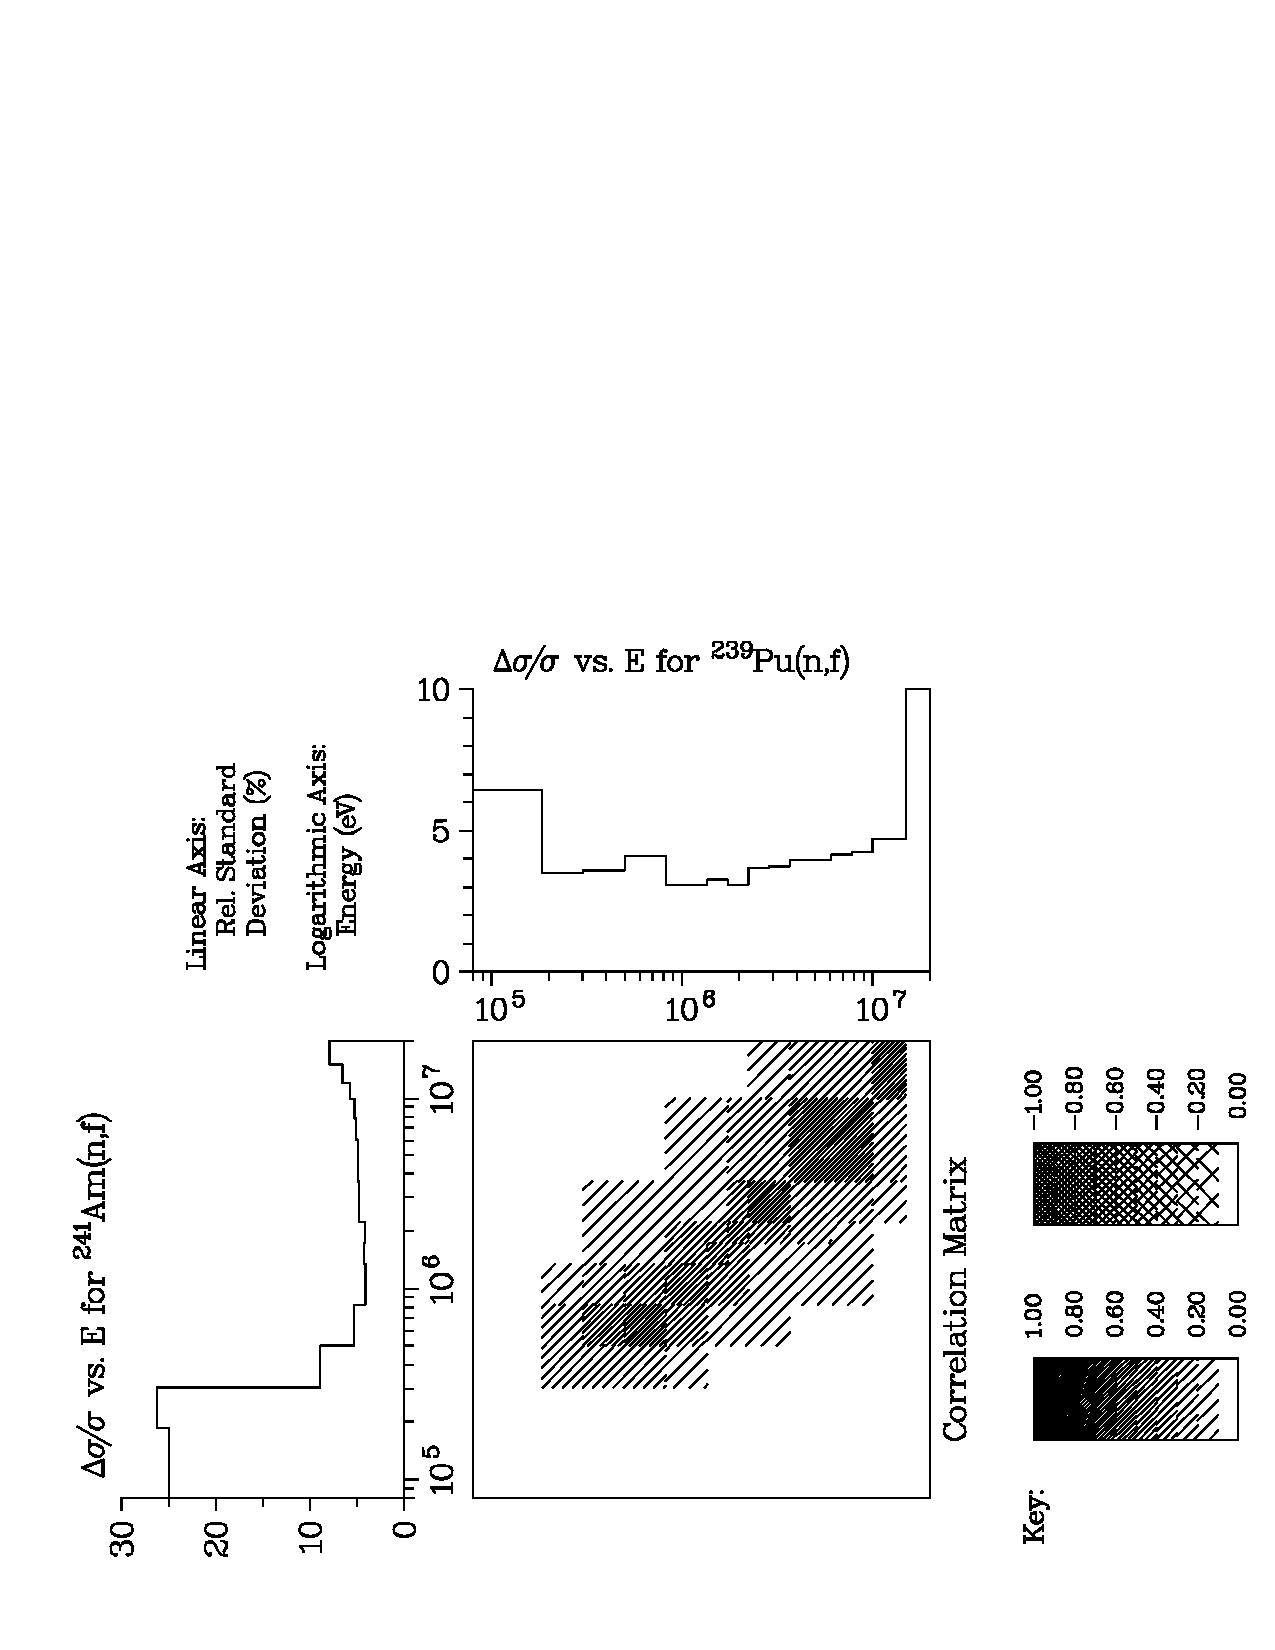
\includegraphics[keepaspectratio, height=5in, angle=270]{figs/errorr2ack}
\caption[Ratioed covariance data for $^{239}$Pu(n,f) and $^{241}$Am(n,f)
 cross sections]{Covariance data for $^{239}$Pu(n,f) with $^{241}$Am(n,f).
 This older figure illustrates the black \& white option for covariance
 plots using hatching to represent levels of correlation.}
\label{ratcov}
\end{figure}

\subsection{Multigroup Processing of Resonance-Parameter Uncertainties}
\label{ssERRORR_MGRR}

In some materials, and in certain energy regions, the cross-section
uncertainty is dominated by the uncertainty in resolved resonance
parameters.  As described above, there are several formats available
in the ENDF-6 format for describing resonance covariances.  When using
the early ENDF-5 format (which is available in the ENDF-6 format as
\cword{LCOMP}=0) the resonance-parameter contribution to the uncertainty
in infinite-dilution fission and capture cross sections is included
automatically when cross-section covariances are processed.  The
contribution is obtained from the Breit-Wigner formulae for the
fission and capture areas of a resonance, $A_f$ and $A_{\gamma}$.
By differentiating these formulae with respect to the resonance
parameters, one obtains a set of sensitivities.  With these
sensitivities and the covariance matrix of the parameters from
MF32, one can apply the propagation-of-errors formula to obtain
the covariances ${\rm cov}(A_{\gamma},A_{\gamma})$,
${\rm cov}(A_{\gamma},A_f)$, and ${\rm cov}(A_f,A_f$).

The resonance contribution is properly weighted with the isotopic
abundance and the ratio of the weight function at the resonance to the
average weight in the group.  It is assumed, however, that the area of
a resonance lies entirely within the group that contains the resonance
energy $E_r$.  Because of this assumption, and because ENDF-5 and the
\cword{LCOMP}=0 option of ENDF-6 provide no correlations between
parameters of different resonances, the calculated resonance-parameter
contribution affects only the diagonal elements of the affected
matrices, ${\rm cov}[X_K(a),X_K(b)]$.

When one of the more advanced options (\cword{LCOMP}=1 or
\cword{LCOMP}=2) is found in MF32, and for Single-Level
Breit-Wigner\index{Single-Level Breit-Wigner!SLBW},
Multi-Level Breit-Wigner\index{Multi-Level Breit-Wigner!MLBW},
or Reich-Moore\index{Reich-Moore!RM} resonance parameters, the
ERRORR code branches to the ERRORJ\index{ERRORJ} logic.  The resonance
cross sections are computed on a special grid and group averaged.  Then
each parameter is changed in turn to generate new cross sections.
Sensitivity parameters are computed from the differences.  These
sensitivity coefficients are then combined with the covariances of
the parameters to obtain covariances on the multigroup cross sections.
The matrices are very large in many cases, and the folding is
time consuming.  There are two formats in use for the parameter
covariances.  One gives each value in a full computer word.  With
many resonances, this can become very bulky.  The other uses a
more compact representation based on the correlations.  Just a few
digits are used for each correlation, thus reducing the size of
the evaluation.  The coding must reconstruct the actual covariance
values before folding them with the sensitivities, so this
economization doesn't help with the time required to fold the
data in the final cross section covariances.

If Reich-Moore-Limited\index{Reich-Moore-Limited!RML} resonances
are found (\cword{LRF}=7, a different branch is taken.  In this case,
it is possible to use analytic formulas to compute the cross section
sensitivities to the parameters.  These formulas are given in detail
in the SAMMY reference\cite{SAMMY}.  These sensitivities are computed
on a special energy grid and group averaged.  They are then folded
with the parameter covariances as described above to obtain the
cross section covariances.


\subsection{Processing of Lumped-Partial Covariances}
\label{ssERRORR_Lump}

The lumped-partial covariance format, allows the evaluator to
specify a group of nuclear reactions and to give the uncertainty only
in the \underline{sum} of the cross sections for that group of
reactions.  One can, for example, replace 30 or 40 discrete-level
inelastic cross sections with 5 or 6 lumped cross sections when
constructing the covariance files.  Because the volume of the
covariance data varies, in general, as the square of the number of
reactions, this lumping can greatly reduce the size of the files.

The first ENDF evaluation to employ the lumped-partial format was
Young's evaluation\cite{Young-2,Young} for $^7$Li (ENDF/B-V, Rev.~2).
All covariance data for this evaluation have been successfully
processed into multigroup form using ERRORR.  The covariances for
\cword{MT854} (a single real level with an excitation energy of
4.63 MeV) with \cword{MT855} (6 lumped pseudo-levels, with excitation
energies ranging from 4.75 MeV to 6.75 MeV) have been plotted in
Fig.~\ref{licov}.  The large negative correlations along the diagonal
result from the fact that, below 10 MeV, these inelastic reactions are
the major contributors to the relatively well-known tritium production
cross section.  An upward variation in one reaction at a given energy
must be accompanied by a downward change in the other reaction.  As shown
in the plot, the magnitude of this negative correlation diminishes at
higher energies, as other reactions begin to contribute significantly to
the tritium-production cross section.  Plots of this type, prepared using
ERRORR and \hyperlink{sCOVRhy}{COVR}, have proved to be
useful tools in the validation of
the covariance files of new evaluations\cite{LaBauve}.

\begin{figure}[thb]\centering
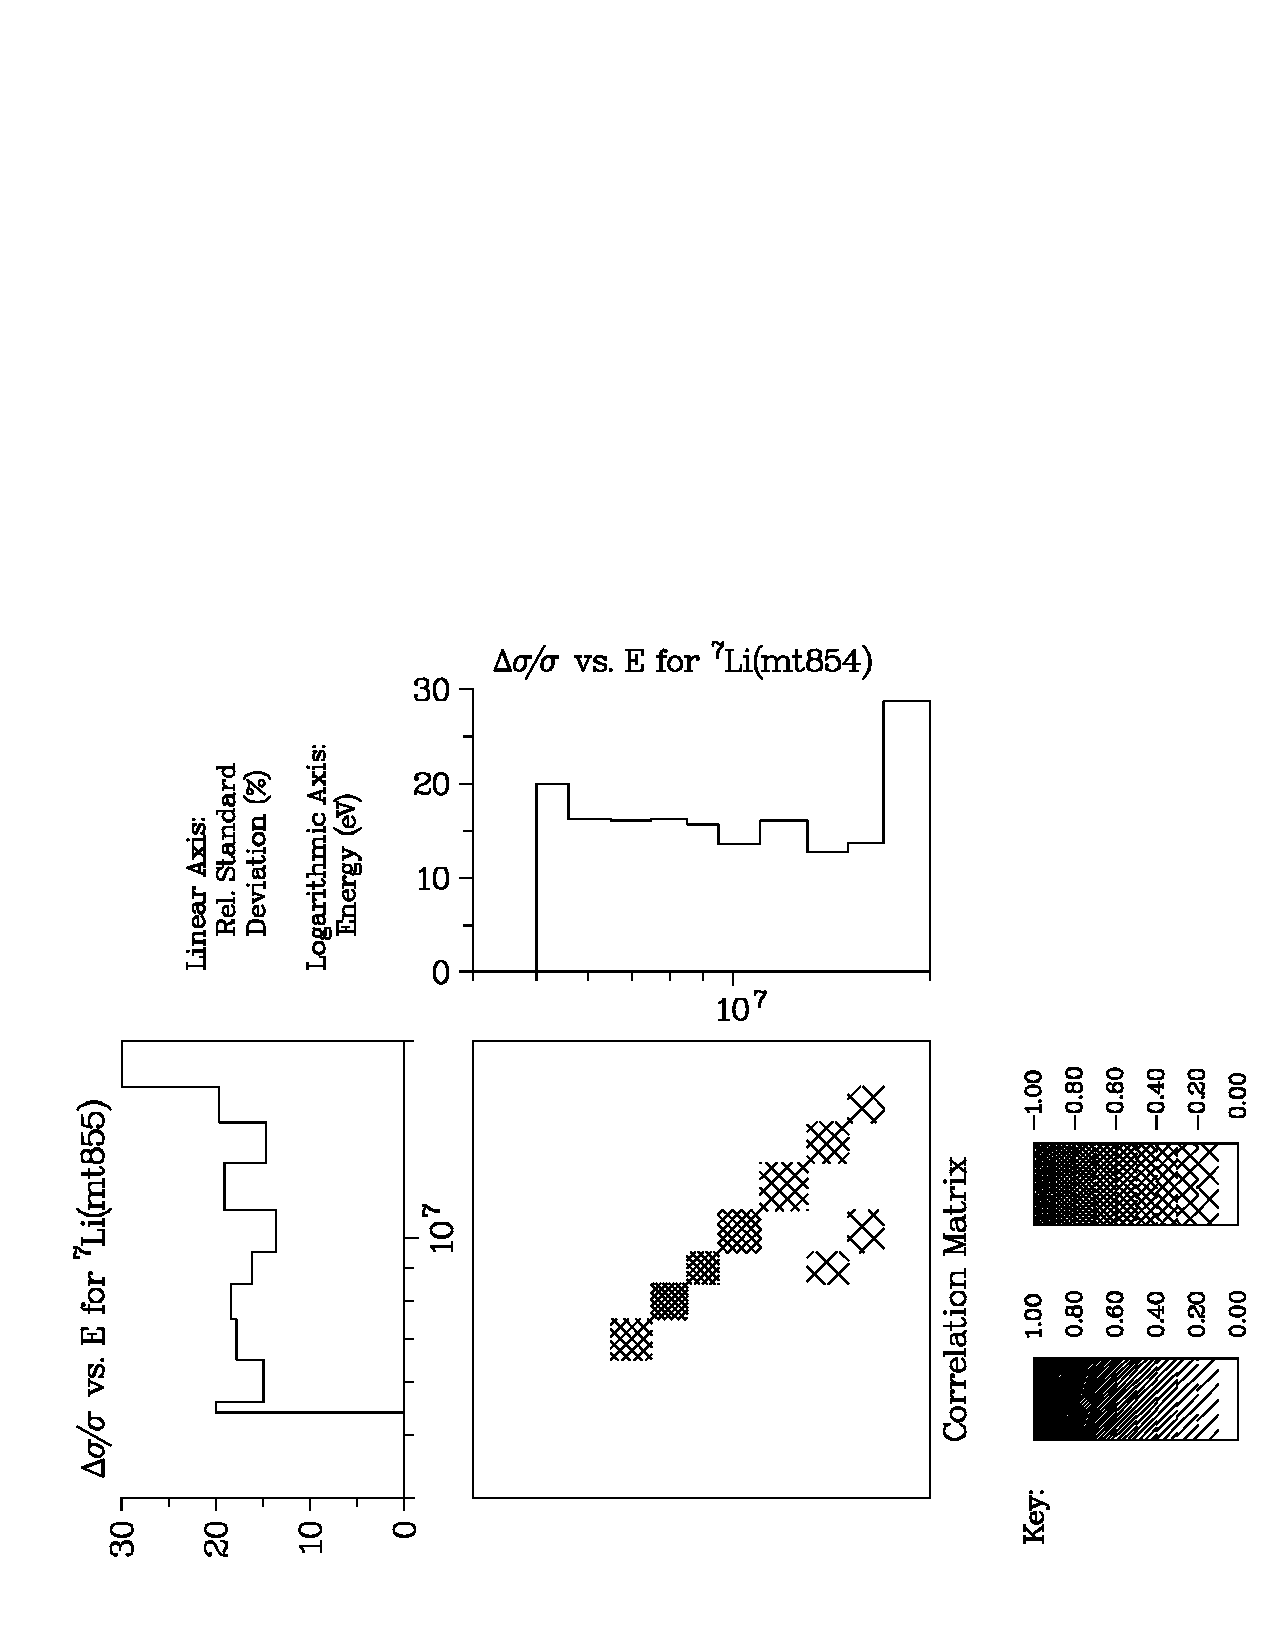
\includegraphics[keepaspectratio, height=5in, angle=270]{figs/errorr3ack}
\caption[$^{7}$Li ``Lumped" covariance data]{Covariance data for $^7$Li
 (MT854) with $^7$Li (MT855).}
\label{licov}
\end{figure}

\subsection{Input Instructions and Sample Input for ERRORR}
\label{ssERRORR_inp}

As an aid to discussions of the user input to ERRORR, we list below the
input instructions that appear as comment cards at the beginning of the
current version of this module.  Since the code and, hence, the
instructions change from time to time, it is always advisable to
consult the comment-card instructions contained in the version of the
code actually being used and not to rely on the instructions published
in any document, including this one.  Note that the word ``tape'' is
used in the instructions to refer to an input or output file,
regardless of the actual storage medium.
\index{ERRORR!ERRORR input}
\index{input!ERRORR}

\newpage
\small
\begin{ccode}

   !---input specifications (free format)---------------------------
   !
   !  card 1
   !    nendf   unit for endf tape
   !    npend   unit for pendf tape
   !    ngout   unit for input group xsec (gendf) tape
   !            (if zero, group xsecs will be calculated)
   !            (if iread eq 2 or if mfcov eq 31, 35 or 40 (see
   !             card 7), then ngout cannot be zero)
   !            (if mfcov eq 35 (see card 7),
   !              ngout cannot be zero)
   !            (default=0)
   !    nout    unit for output covariance tape (default=0)
   !    nin     unit for input covariance tape (default=0)
   !            (nin and nout must be both coded or both binary)
   !    nstan   unit for ratio-to-standard tape (default=0)
   !  card 2
   !    matd    material to be processed
   !    ign     neutron group option
   !            (ign definition same as groupr, except ign=19,
   !            which means read in an energy grid, as in ign=1,
   !            and supplement this with the endf covariance grid
   !            within the range of the user-specified energies)
   !            (default=1)
   !    iwt     weight function option (default=6)
   !    iprint  print option (0/1=minimum/maximum) (default=1)
   !    irelco  covariance form (0/1=absolute/relative) (default=1)
   !  card 3    (*** REQUIRED for njoy2012 and later ***)
   !    mprint  print option for group averaging (0/1=min (default)/max)
   !    tempin  temperature (default=300)
   !
   !---for endf/b version 4 (iverf=4) only--------------------------
   !
   !  card 4
   !    nek     number of derived xsec energy ranges
   !            (if zero, all xsecs are independent)
   !  card 5    (omit if nek=0)
   !    ek      nek+1 derived xsec energy bounds
   !  card 6    (omit if nek=0)
   !    akxy    derived cross section coefficients, one row/line
   !
   !---for endf/b version 5 or 6 (iverf=5 or 6) only------------------------
   !
   !  card 7
   !    iread   0/1/2=program calculated mts/input mts and eks/
   !            calculated mts plus extra mat1-mt1 pairs from input
   !            (default=0)
   !    mfcov   endf covariance file (31, 33, 34, 35 or 40) to be
   !            processed (default=33).
   !            note--contribution to group cross section
   !            covariances from resonance-parameter uncertainties
   !            (mf=32) is included when mfcov=33 is specified.
   !            (mf=-33) high speed calc for test case
   !            (mf=333) hight speed calc for test case (faster)
   !    irespr  processing for resonance parameter covariances
   !            (mf=32) (default=1)
   !            0 = area sensitivity method
   !            1 = 1\% sensitivity method
   !    legord  legendre order for calculating covariances (default=1)
   !            (if mfcov is not 34, legord is ignored)
   !    ifissp  subsection of the fission spectrum covariance
   !            matrix to process (default=-1 which means process
   !            the subsection that includes efmean).  The value
   !            for ifissp that appears in njoy's standard output
   !            will equal the subsection containing efmean.
   !            (if mfcov is not 35, ifissp is ignored)
   !    efmean  incident neutron energy (eV).  Process the covar-
   !            iance matrix subsection whose energy interval in-
   !            cludes efmean.  if ifissp=-1 and efmean is not
   !            specified, set efmean=2.e6_kr.  But if there is only
   !            one subsection, process it and if the input efmean
   !            was not within this subsection's energy range then
   !            redefine efmean to equal the average energy for
   !            this subsection.
   !            (if mfcov is not 35, efmean is ignored)
   !    dap     user specified scattering radius uncertainty, given
   !            as a fraction (i.e., dap=0.1 means 10\% uncertainty
   !            in the scattering radius).  The default value is
   !            zero.  This variable is only defined for mfcov=33
   !            and if non-zero will be used in lieu of any data
   !            that might have been read from the nendf tape.
   !
   !  following cards only if iread eq 1
   !  card 8
   !    nmt     no. mts to be processed
   !    nek     no. derived cross section energy ranges
   !            (if zero, all xsecs are independent)
   !  card 8a
   !    mts     nmt mts
   !  card 8b   (omit if nek=0)
   !    ek      nek+1 derived cross section energy bounds
   !  card 9    (omit if nek=0)
   !    akxy    derived cross section coefficients, one row/line
   !
   !  following card only if iread eq 2
   !  card 10
   !    mat1    cross-material reaction to be added to
   !    mt1         covariance reaction list.
   !            repeat for all mat1-mt1 pairs desired
   !            terminate with mat1=0.
   !
   !  following card only if nstan ne 0
   !  card 11
   !    matb    standards reaction referenced
   !    mtb         in matd.
   !    matc    standards reaction to be
   !    mtc         used instead.
   !            repeat for all standard reactions to be redefined.
   !            terminate with matb=0.
   !  note.  if matb(1) and mtb(1) are negative, then matc(1) and
   !    mtc(1) identify a third reaction, correlated with matd thru
   !    the use of the same standard.  covariances of all reactions
   !    in matd (which reference the standard) with the reaction
   !    matc(1)-mtc(1) will be produced.  the standard reaction
   !    must be identified on card 10 and repeated as the negative
   !    entries on card 11.  the group xsec tape ngout must include
   !    all covariance reactions in matd, plus matc(1)-mtc(1).
   !
   !  card 12a (for ign eq 1 or ign eq 19)
   !    ngn     number of groups
   !  card 12b
   !    egn     ngn+1 group bounds (ev)
   !  card 13 (for iwt eq 1 only)
   !    wght    weight function as a tab1 record
   !  card 13b  analytic flux parameters (iwt=4 only)
   !    eb      thermal break (ev)
   !    tb      thermal temperature (ev)
   !    ec      fission break (ev)
   !    tc      fission temperature (ev)
   !
   ! ---options for input variables------------------------------------
   !
   !      ign          meaning
   !      ---          -------
   !       1           arbitrary structure (read in)
   !       2           csewg 239-group structure
   !       3           lanl 30-group structure
   !       4           anl 27-group structure
   !       5           rrd 50-group structure
   !       6           gam-i 68-group structure
   !       7           gam-ii 100-group structure
   !       8           laser-thermos 35-group structure
   !       9           epri-cpm 69-group structure
   !      10           lanl 187-group structure
   !      11           lanl 70-group structure
   !      12           sand-ii 620-group structure
   !      13           lanl 80-group structure
   !      14           eurlib 100-group structure
   !      15           sand-iia 640-group structure
   !      16           vitamin-e 174-group structure
   !      17           vitamin-j 175-group structure
   !      18           xmas 172-group structure
   !      19           read in, supplemented with endf covariance grid
   !
   !      iwt          meaning
   !      ---          -------
   !       1           read in smooth weight function
   !       2           constant
   !       3           1/e
   !       4           1/e + fission spectrum + thermal maxwellian
   !       5           epri-cell lwr
   !       6           (thermal) -- (1/e) -- (fission + fusion)
   !       7           same with t-dep thermal part
   !       8           thermal--1/e--fast reactor--fission + fusion
   !       9           claw weight function
   !      10           claw with t-dependent thermal part
   !      11           vitamin-e weight function (ornl-5505)
   !      12           vit-e with t-dep thermal part
   !
   !--------------------------------------------------------------------

\end{ccode}
\normalsize

As an example of the use of these commands, here is the input used
to produce Fig.~\ref{b10cov}, the covariance plot for $^{10}$B
from ENDF/B-VII.0.

\small
\begin{ccode}

    1. errorr
    2. 31 32 0 33/
    3. 525 3 9 1 1/
    4. 0 0./
    5. 0 33/
    6. covr
    7. 33 0 34/
    8. 1/
    9. /
   10. /
   11. 525/
   12. viewr
   13. 34 35/
   14. stop

\end{ccode}
\normalsize

\noindent
The line numbers are for reference and are not part of the input.
Identical versions of the ENDF/B-VII.0 file for $^{10}$B can be
copied to \cword{tape31} and \cword{tape32}.  The ERRORR output
will appear on \cword{tape33}.  In this sample input deck, that file
is the input file to \hyperlink{sCOVRhy}{COVR} which
generates the plot instructions that are subsequently written to
\cword{tape34}.  Line 3 defines the material to be
processed (525, or $^{10}$B), the group structure, the weight function,
the listing option, and requests relative covariances.  Line 4 turns
off printing for the group averaging and requests zero temperature.
Users are cautioned that line 4 is now required in all ERRORR input decks
whereas in njoy99 it is only required when ngout is zero.  Line 5
asks the program to calculate the MT numbers to be processed
and to work with File 33.  The \hyperlink{sCOVRhy}{COVR} and
\hyperlink{sVIEWRhy}{VIEWR} input in lines 6 through
13 act to prepare the graph as seen in Fig.~\ref{b10cov}.

The follwing paragraphs give more detail on how the various
input parameters are used.

\cword{npend, ngout } \ldots\hspace{.1in}The user must supply either a
PENDF\index{PENDF} tape on unit \cword{npend} or a GENDF\index{GENDF}
tape on unit \cword{ngout}.  If present, the \cword{npend} tape should
contain pointwise (resonance-reconstructed, but not multigrouped) data
and is normally produced with the
\hyperlink{sRECONRhy}{RECONR}\index{RECONR} module.  If the
resonance region is of no interest, a simple copy of the ENDF tape will
suffice for this purpose.  The GENDF tape, if present, should contain
multigroup cross sections and/or $\overline{\nu}$ values, produced by
the \hyperlink{sGROUPRhy}{GROUPR}\index{GROUPR} module,
for all reactions for which multigroup
covariances are needed.  Group cross sections need not be in the same group
structure as the requested output covariances, although if the input
group structure is much coarser than the output structure, rather crude
approximations will be made in deriving an effective set of fine-group
cross sections and fluxes from the coarse input data.  Certain types
of covariance calculations related to fission data or the computation
of cross-material covariances require the user to supply a GENDF
tape on \cword{ngout} (that is, \cword{npend} must be zero).

\cword{nin, nout } \ldots\hspace{.1in}Input and output covariance
tapes in the user's group structure may either be both formatted or
both binary.  Although ERRORR lacks an explicit multimaterial
loop, the same effect can be achieved by executing a series of ERRORR
runs, with the output of one run becoming the input of the next.  Only
two unit numbers need be employed, with the data going back and forth
between them until the multimaterial library is complete.  To save
time, binary files should be used for this
purpose.  \hyperlink{sMODERhy}{MODER}\index{MODER}
can be used to convert the final output tape from binary to formatted
form, if desired.

\cword{nstan } \ldots\hspace{.1in}This tape is needed if covariances
are requested for a reaction pair that is related by ratio
measurements, as discussed in Section~\ref{ssERRORR_Ratio}.  The ENDF
subsection for
such a pair will contain an NC-type sub-subsection with
\cword{LTY}=1, 2, or 3.  The specific pairs in ENDF/B-V that require
a standards tape are tabulated  in Table~\ref{ratios}
(Section~\ref{ssERRORR_Ratio}).
For other evaluations, one can assume \cword{nstan} is not needed.
The code will stop with a clear error message if this assumption
proves incorrect.

\cword{iread } \ldots\hspace{.1in}For ENDF/B versions 5 and 6, the list of
reactions for which covariances are produced is constructed in one of
several ways, depending on the value of \cword{iread}.  If
\cword{iread}=0, which is the generally recommended choice,
the reaction list is assumed to be identical to the list of sections
contained in the ENDF/B covariance file (see \cword{mfcov} below).
Although \cword{iread}=0 is the most convenient option for constructing
the list of covariance reactions, it leads to a problem if some
covariance reactions have thresholds above the highest group boundary
of the user's structure.  These reactions will have zero cross sections
in all groups and thus will be omitted from \cword{ngout}.  To avoid
this difficulty, ERRORR automatically resets the user's highest group
boundary to 20 MeV whenever \cword{iread}=0.  By judicious choice of
weighting functions, one can minimize the effect of this resetting on
the other cross sections and their covariances.

If \cword{iread}=1, only the covariance reactions specifically
named by the user will be included in the reaction list.  For certain
applications, this option can save considerable execution time.
However, to take advantage of this option, the user must examine the
ENDF evaluation visually to determine which reactions are derived
from other reactions in each energy region.  As discussed in
Section~\ref{ssERRORR_Str}, this information is contained in NC-type
sub-subsections
with \cword{LTY}=0.  Incorrect results will be obtained if one requests
processing for a given reaction without processing all of the reactions
from which the given reaction is derived in the energy region spanned
by the output group structure.  The inclusion of those reactions may
require, in turn, additional inclusions as well.  In addition, the user
must extract from the file (and enter into the input) the appropriate
derivation coefficients and the energy ranges over which they
apply.  An example of the required input is presented below in the
discussion of the parameters \cword{nmt}, \cword{nek}, \cword{mts},
\cword{ek}, and \cword{akxy}.

If \cword{iread}=0 or 1, a complete set of covariance matrices
is written.  That is, covariance matrices are produced for
every reaction-pair combination that can be formed from the
given reaction list.  For those reaction pairs where the evaluator has
not specified the covariances, the output matrix contains only zeros.

In the evaluation containing cross-material covariances, subsections
involving the other materials will be ignored if \cword{iread}=0 or
1.  These subsections can be selectively processed by
specifying \cword{iread}=2.  If \cword{iread}=2, the reaction list is
initially constructed in the same way as for \cword{iread}=0.  This
list is then supplemented with a list of extra reactions (MAT1$_k$,
MT1$_k$) (where (MAT1$_k$ $\neq$ MATD), specified by the user.  The
output in this case contains matrices for all of the (MATD, MT$_i$;
MATD,,MT$_j$) combinations, as before, plus matrices for all
(MATD, MT$_i$; MAT1$_k$, MT1$_k$) combinations.  However, covariances
among the extra reactions, for example (MAT1$_k$, MT1$_k$;
MAT1$_m$,,MT1$_m$), are not computed.  Input for an example problem that
illustrates the use of \cword{iread}=2 is given below, in the
discussion of \cword{mfcov}.  That discussion also includes an
illustration of the set of MAT/MT combinations that
are processed when \cword{iread}=2.

\cword{mfcov} \ldots\hspace{.1in} is used to specify whether
covariances of $\overline{\nu}$ (\cword{mfcov}=31), cross
sections (\cword{mfcov}=33), angular distributions (\cword{mfcov}=34),
secondary energy distributions (\cword{mfcov}=35), or radioactive nuclide
production (\cword{mfcov}=40) are needed.  If \cword{mfcov}=31, 35, or 40,
it is necessary to supply multigrouped
cross sections and $\overline{\nu}$ values on a GENDF tape
that is, \cword{npend} must be 0); the sample problem below shows
the calculational sequence required.  The parameter \cword{mfcov}=32
is reserved for a planned future capability to compute
uncertainties in self-shielded cross sections.  If \cword{mfcov=33},
the contribution of the uncertainty in individual resonance parameters
(File 32) is included in the calculated uncertainty in
infinite-dilution group cross sections.  Given below is the complete
NJOY input for a calculation of a multigroup $\overline{\nu}$
covariance library for $^{238}$U, including five cross-material
reactions.

\small
\begin{ccode}

   moder / mount ENDF tapes 515, 516, and 555 on units 20, 21, and 22.
   1 -23/
   'ENDF/B-V NUBAR COVARIANCE MATERIALS'/
   20 1380/
   20 1381/
   21 1390/
   22 1395/
   22 1398/
   20 1399/
   0/
   moder / copy ENDF for use as a PENDF.
   -23 -24/
   groupr / prepare GENDF with multigrouped nubars.
   -23 -24 0 25/
   1380 3 0 3 0 1 1 0/
   'BIG3 + 2 NUBAR'/
   0./
   1.e10/
   3 452 'TOTAL NUBAR'/
   0/
   1381/
   3 452 'TOTAL NUBAR'/
   0/
   1390/
   3 452 'TOTAL NUBAR'/
   0/
   1395/
   3 452 'TOTAL NUBAR'/
   0/
   1398/
   3 452 'TOTAL NUBAR'/
   3 455 'DELAYED NUBAR'/
   3 456 'PROMPT NUBAR'/
   0/
   1399/
   3 452 'TOTAL NUBAR'/
   0/
   0/
   errorr / prepare multigroup nubar covariance library.
   -23 0 25 26/
   1398 19 1 1/
   0 0. /
   2 31/
   1380 452/
   1381 452/
   1390 452/
   1395 452/
   1399 452/
   0/
   1/
   1.e7 1.7e7/
   stop

\end{ccode}
\normalsize

Note the use of the \hyperlink{sMODERhy}{MODER} module
to prepare a special ENDF tape
containing selected evaluations from other ENDF tapes.  Because only
high-energy $\overline{\nu}$ data are requested (10 -- 17 MeV), it is
unnecessary to use \hyperlink{sRECONRhy}{RECONR} to prepare
a PENDF tape for \hyperlink{sGROUPRhy}{GROUPR}.  A copy
of the ENDF tape is used instead.

Following the prescription given in the discussion of the
\cword{iread}=2 option, with this particular input, covariance matrices
will be produced for those reaction pairs marked with an X in
Table~\ref{pairs}.  The remaining non-redundant possibilities (dashes)
can be filled in with successive ERRORR runs with
\cword{MATD}=1380, 1381, etc.

\begin{table}[t]
\caption{Reaction pairs in the ENDF/B-V $^{238}$U evaluation}
\label{pairs}
\begin{center}
\begin{tabular}{|l|c|c|c|c|c|c|c|c|c|}
\hline
    & a  &  b  &  c  &  d  &  e  &  f  &  g  &  h  & i \\ \cline{1-10}
a = (1398,452) &  X  &  X  &  X  &  X  &  X  &  X  &  X  &  X  &  X \\
b = (1398,455) &  &  X  &  X &  X  &  X  &  X  &  X  &  X  &  X \\
c = (1398,456) &  &  &  X &  X  &  X  &  X  &  X  &  X  &  X  \\
d = (1380,452) &  &  &  &  -- &  -- &  --  &  -- &  -- &  -- \\
e = (1381,452) &  &  &  &     &  -- &--  &  -- &  -- &  -- \\
f = (1390,452) &  &  &  &     &     &  --  &  -- &  -- &  -- \\
g = (1395,452) &  &  &  &     &     &      &  -- &  -- &  --  \\
h = (1398,452) &  &  &  &     &     &      &     &  -- &  --  \\
i = (1399,452) &  &  &  &     &     &      &     &     &  -- \\
\cline{1-10}
\end{tabular}
\end{center}
\end{table}

\cword{nwt}, \cword{nek}, \cword{mts}, \cword{ek}, \cword{akxy}
\ldots\hspace{.1in}
For ENDF/B version 5, if \cword{iread}=1, the user specifies a subset of the
evaluator's covariance reactions (that is, a subset of the sections
of \cword{mfcov}), as the particular set of reactions for which
processing is requested.  These \cword{nmt} desired reactions are
entered in the array \cword{mts}.  As mentioned in the discussion of
\cword{iread} above, one must also include in the \cword{mts} array all
reactions from which the desired reactions are derived.

Another requirement of the \cword{iread}=1 option is that the actual
derivation coefficients, called \cword{akxy} in the code, but called
$C_I(a,c)$ in the discussion in Section~\ref{ssERRORR_summ}, must be
entered in the
ERRORR input for \cword{nek} energy ranges spanning the output group
structure.  Adjacent ENDF derivation ranges may be merged into a
single range if the derivation-coefficient matrix for the \cword{nmt}
explicitly requested reactions is the same in each of the adjacent
ranges.  The ordering of the $C_I(a,c)$ data is as follows: on one line
of input the coefficients are specified for a fixed $a$-value and for
all $c$-values ranging from 1 to \cword{nmt}.  One such line is given
for each $a$-value.  Finally, there is an outer loop over the
\cword{nek} energy ranges.  An example of the input that is required
for \cword{iread}=1 is given below for the case of ENDF/B-V carbon
\cword{MAT}=1306.  It will be necessary to examine File 33 of the
evaluation (which is available on the ENDF/B-V standards file, Tape
511), in order to understand the details of this example.

\small
\begin{ccode}

   moder
   20- 21/
   moder / copy ENDF for use as a PENDF.
   -21 -22/
   errorr
   -21 -22 0 -23/
   1306 3 1/
   2 0 0/
   1 33/
   7 3/
   1 2 4 102 103 104 107/
   1.e-5 2e6 4.812e6 2e7/
   0 1 0 1 0 0 0/
   0 1 0 0 0 0 0/
   0 0 1 0 0 0 0/
   0 0 0 1 0 0 0/
   0 0 0 0 1 0 0/
   0 0 0 0 0 1 0/
   0 0 0 0 0 0 1/
   1 0 0 0 0 0 0/
   0 1 0 0 0 0 0/
   0 0 1 0 0 0 0/
   0 0 0 1 0 0 0/
   0 0 0 0 1 0 0/
   0 0 0 0 0 1 0/
   0 0 0 0 0 0 1/
   1 0 0 0 0 0 0/
   0 1 0 0 0 0 0/
   1 -1 0 -1 -1 -1 -1/
   0 0 0 1 0 0 0/
   0 0 0 0 1 0 0/
   0 0 0 0 0 1 0/
   0 0 0 0 0 0 1/
   stop

\end{ccode}
\normalsize

Note that here, even if the user wanted to process only M=2 and
MT=4, for example, it is nevertheless necessary to include
MT=1, MT=102, MT=103, MT=104, and MT=107, because the \cword{ign}=3
group structure extends to 17.0 MeV, and above 4.812 MeV, MT=4 is
derived from the relation
\begin{equation}
\sigma_4 = \sigma_1 - \sigma_2 - \sigma_{102} - \sigma_{103} -
\sigma_{104} - \sigma_{107} \; .
\end{equation}
See the corresponding $C_I(a,c)$ matrix in the input above (the
last 7 lines before \cword{stop}).

\cword{matb}, \cword{mtb}, \cword{matc}, \cword{mtc} \ldots\hspace{.1in}Card 11
provides a capability to remap all references to a given standards reaction
\cword{(matb, mtb)} appearing in NC-type sub-subsections with
\cword{lty}=1, 2, or 3 into references to a different
reaction \cword{(matc, mtc)}.  (See the discussion of ratio measurements
in Section~\ref{ssERRORR_Ratio}.)  This facility is useful if the evaluation
\cword{(matb, mtb)} is for some reason unavailable.  Up to 5 such
standards can be redefined.  As explained in the note on the input
instructions at the beginning of this section, Card 11 is also used, if
\cword{matb(1)} and \cword{mtb(1)} are negative, to process covariances
between two distinct reactions, both measured relative to a common
standards reaction.  This was referred to as the \cword{lty}=4 case
in Section~\ref{ssERRORR_Ratio}.  A separate ERRORR run is required for
each requested \cword{lty}=4 reaction pair.

This second use of Card 11 is illustrated in the sample NJOY input
listed below, which is the input used to generate and plot the
data shown in Fig.~\ref{ratcov}.  The input to the
\hyperlink{sCOVRhy}{COVR}\index{COVR}
module contained in the sample is explained in the following chapter.

\small
\begin{ccode}

   mount T562 on tape30
   mount T563 on tape40
   mount T560 on tape50

   moder
   1 -31/
   'U235 FROM T562'/
   30 1395/
   0/
   moder
   1 -21/
   'AM241 FROM T560 AND PU239 FROM T563'/
   50 1361/ AM241
   40 1399/ PU239
   0/
   reconr
   -21 -22/
   '10 PERCENT PENDF FOR AM241 AND PU239'/
   1361/
   .1/
   1399/
   .1/
   0/
   GROUPR
   -21 -22 0 -24/
   1361 3 0 2 0 1 1 0/
   '30 GROUP XSECS FOR AM241 AND PU239'/
   0/
   1e10/
   3 1/
   3 2/
   3 4/
   3 16/
   3 17/
   3 18/
   3 102/
   0/
   1399
   3 18/
   3 102/
   0/
   0/
   errorr
   -21 0 -24 -25 0 -31/
   1361 3 1 1/
   0 0. /
   0 33/
   0/
   errorr
   -21 0 -24 -28 -25 -31/
   1399 3 1 1/
   0 0. /
   2 33/
   1395 18/
   0/
   -1395 -18 1361 18/
   0/
   covr
   -28/
   0 0 0 8e4/
   1 1 0 0 2/
   1399 18 1361 18/
   stop

\end{ccode}
\normalsize

The input for a File 34 case preparing covariances for an angular
distribution is shown below.  This is the input that produced
Fig.~\ref{mf34cov} shown above.  This deck runs a job sequence
that includes \hyperlink{sMODERhy}{MODER} (ASCII-to-binary
conversion), \hyperlink{sRECONRhy}{RECONR} and
\hyperlink{sBROADRhy}{BROADR} (cross section reconstruction
to 300K), \hyperlink{sGROUPRhy}{GROUPR}
(unweighted, infinitely dilute multigroup cross sections plus
average $\bar{\mu}$), ERRORR (specifying \cword{mfcov}=34 for
$\bar{\mu}$ covariance processing), and
\hyperlink{sCOVRhy}{COVR} and \hyperlink{sVIEWRhy}{VIEWR} (for plot
generation and conversion to Postscript format).  The input on
\cword{tape20} was the JENDL-3.3 evaluation for $^{238}$U.

\small
\begin{ccode}

   moder
    20 -21 /
   reconr
    -21 -22 /
    'processing jendl-3.3 u-238.'/
    9237 0 0 /
    0.001 /
    0 /
   broadr
    -21 -22 -23 /
    9237 1 0 0 0 /
    0.001 /
    300. /
    0 /
   groupr
    -21 -23 0 91 /
    9237 3 0 2 1 1 1 0 /
    'test'/
    300. /
    1.0e10 /
    3 /
    3 251 'mubar' /
    0 /
    0 /
   --
   -- process mf34
   errorr
    -21 0 91 27 0 0 /
    9237 3 2 1 1 /
    0 300. /
    0 34 1 1 -1 /
   --
   -- make mf34 plot file.
   covr
    27 0 37 /
    1 /
    /
    /
    9237 /
   --
   -- make mf34 postscript file.
   viewr
    37 47 /
   stop

\end{ccode}
\normalsize

The input for the File 35 case that produced the plot of secondary
energy covariances seen in Fig.~\ref{mf35cov} is given below.
This is a problem taken from the NJOY test suite that uses a
fictitious input file for $^{252}$Cf.  The
\hyperlink{sGROUPRhy}{GROUPR} and ERRORR
inputs specify a user-defined group structure that corresponds to
the energies listed in File 1 of the evaluation with the
uncertainties provided by the evaluator.  This makes it easy
to verify that the results agree with the evaluator's intent.

\small
\begin{ccode}

   --
   -- Copy ascii input to binary.
   moder
    20 -21 /
   --
   -- Resonance reconstruction, to 0.1\%.
   reconr
    -21 -22 /
    'processing e70 252Cf with decay mf5/mt18 & mf35/mt18'/
    9999 0 0 /
    0.001 /
    0 /
   --
   -- Doppler broaden to 300K.
   broadr
    -21 -22 -23 /
    9999 1 0 0 0 /
    0.001 /
    300. /
    0 /
   --
   -- Group average, 300K with mf35 group structure.
   --  - All file 3 cross sections plus fission spectrum.
   groupr
    -21 -23 0 91 /
    9999 1 0 2 1 1 1 1 /
    'test'/
    300. /
    1.0e10 /
    71 / # of groups, energy boundaries follow:
    1.000000-5 1.500000+4 3.500000+4 5.500000+4 7.500000+4
    9.500000+4 1.150000+5 1.350000+5 1.650000+5 1.950000+5
    2.250000+5 2.550000+5 3.050000+5 3.550000+5 4.050000+5
    4.550000+5 5.050000+5 5.550000+5 6.050000+5 6.550000+5
    7.050000+5 7.550000+5 8.050000+5 8.550000+5 9.050000+5
    9.550000+5 1.050000+6 1.150000+6 1.250000+6 1.350000+6
    1.450000+6 1.550000+6 1.650000+6 1.750000+6 1.850000+6
    1.950000+6 2.150000+6 2.350000+6 2.550000+6 2.750000+6
    2.950000+6 3.250000+6 3.550000+6 3.850000+6 4.150000+6
    4.450000+6 4.750000+6 5.050000+6 5.550000+6 6.050000+6
    6.550000+6 7.050000+6 7.550000+6 8.050000+6 8.550000+6
    9.050000+6 9.550000+6 1.005000+7 1.055000+7 1.105000+7
    1.155000+7 1.205000+7 1.255000+7 1.305000+7 1.355000+7
    1.405000+7 1.460000+7 1.590000+7 1.690000+7 1.790000+7
    1.910000+7 2.000000+7/
    3 /
    5 18  'chi' /
    0 /
    0 /
   --
   -- ERRORJ, mf35
   errorr
    20 0 91 28 0 0 /
    9999 1 2 1 1 /
    0 300. /
    0 35 1 1 -1 1.23e6 /
    71 / # of groups, energy boundaries follow:
    1.000000-5 1.500000+4 3.500000+4 5.500000+4 7.500000+4
    9.500000+4 1.150000+5 1.350000+5 1.650000+5 1.950000+5
    2.250000+5 2.550000+5 3.050000+5 3.550000+5 4.050000+5
    4.550000+5 5.050000+5 5.550000+5 6.050000+5 6.550000+5
    7.050000+5 7.550000+5 8.050000+5 8.550000+5 9.050000+5
    9.550000+5 1.050000+6 1.150000+6 1.250000+6 1.350000+6
    1.450000+6 1.550000+6 1.650000+6 1.750000+6 1.850000+6
    1.950000+6 2.150000+6 2.350000+6 2.550000+6 2.750000+6
    2.950000+6 3.250000+6 3.550000+6 3.850000+6 4.150000+6
    4.450000+6 4.750000+6 5.050000+6 5.550000+6 6.050000+6
    6.550000+6 7.050000+6 7.550000+6 8.050000+6 8.550000+6
    9.050000+6 9.550000+6 1.005000+7 1.055000+7 1.105000+7
    1.155000+7 1.205000+7 1.255000+7 1.305000+7 1.355000+7
    1.405000+7 1.460000+7 1.590000+7 1.690000+7 1.790000+7
    1.910000+7 2.000000+7/
   --
   -- make plot file.
   covr
    28 0 38 /
    1 /
    1.e3 /
    /
    9999 /
   --
   -- make postscript file.
   viewr
    38 39 /
   stop
\end{ccode}
\normalsize

The final example gives the input used to prepare Fig.~\ref{mf40cov}
showing the uncertainties in radionuclide production for $^{93}$Nb.
This is a fairly elaborate input deck, as it includes
\hyperlink{sGROUPRhy}{GROUPR}/ERRORR/
\hyperlink{sCOVRhy}{COVR}/\hyperlink{sVIEWRhy}{VIEWR}
processing for both File 3 and File 10.

\small
\begin{ccode}

   -- Extract/convert neutron evaluated data
   moder
    1 -21/
    '41-Nb-93 from e70'/
    20 4125/
    0/
   --
   -- Make an ASCII copy
   moder
    -21 41 /
   --
   -- Reconstruct xs
   reconr
    41 42/
    'pendf for 41-Nb-93'/
    4125 2/
    0.001 0. 0.003/
    '41-Nb-93 from e70'/
    'Processed with NJOY'/
    0/
   --
   -- Doppler broaden xs
   broadr
    41 42 43/
    4125 1 0 0 0./
    0.001 2.0e6 0.003/
    300./
    0/
   --
   -- groupr, process all file 3 reactions:
   groupr
    41 43 0 44 /
    4125 1 0 6 0 1 1 1 /
    '41-Nb-93 from e70 with NJOY'/
    300. /
    1.e10 /
    21 /
    1.e-5 0.625 10.7 100.0 1.e3 1.e4 1.e5 1.e6
    2.e6 3.e6 4.e6 5.e6 6.e6 7.e6 8.e6 9.e6 10.e6
    12.e6 14.e6 16.e6 18.e6 20.e6 /
    3 /
    0/
    0/
   --
   -- errorj, process all file 3 reaction uncertainties:
   errorr
    41 43 44 45/
    4125 1 6 1 1 /
    0 300. /
    0 33 /
    21 /
    1.e-5 0.625 10.7 100.0 1.e3 1.e4 1.e5 1.e6
    2.e6 3.e6 4.e6 5.e6 6.e6 7.e6 8.e6 9.e6 10.e6
    12.e6 14.e6 16.e6 18.e6 20.e6 /
   --
   -- create plot of mf33 uncertainty data
   covr
    45 0 55 /
    1 /
    1.e-1 /
    /
    4125 /
   viewr
    55 65 /
   --
   -- groupr, process all file 10 reactions:
   groupr
    41 43 0 46 /
    4125 1 0 6 0 1 1 1 /
    '41-Nb-93 from e70 with NJOY'/
    300. /
    1.e10 /
    21 /
    1.e-5 0.625 10.7 100.0 1.e3 1.e4 1.e5 1.e6
    2.e6 3.e6 4.e6 5.e6 6.e6 7.e6 8.e6 9.e6 10.e6
    12.e6 14.e6 16.e6 18.e6 20.e6 /
    10 /
    0/
    0/
   --
   -- errorj, process all file 10 reaction uncertainties:
   errorr
    41 43 46 47/
    4125 1 6 1 1 /
    0 300. /
    0 40 /
    21 /
    1.e-5 0.625 10.7 100.0 1.e3 1.e4 1.e5 1.e6
    2.e6 3.e6 4.e6 5.e6 6.e6 7.e6 8.e6 9.e6 10.e6
    12.e6 14.e6 16.e6 18.e6 20.e6 /
   --
   -- create plot of mf40 uncertainty data
   covr
    47 0 57 /
    1 /
    1.e3 /
    /
    4125 /
   viewr
    57 67 /
   stop

\end{ccode}
\normalsize

\subsection{ERRORR Output File Specification}
\label{ssERRORR_Out}

The results from ERRORR are written to an output file on unit
\cword{nout}, provided that the input parameter \cword{nout} is
nonzero.  This file contains the user's group structure, the
multigroup cross sections, and either absolute (\cword{irelco}=0) or
relative (\cword{irelco}=1) covariances.  If \cword{nout} is positive,
then a formatted (card-image) file is written, and, if negative, a
binary file is written.  In either case, the output is written with the
standard \hyperlink{sNJOYhy}{NJOY} I/O utilities, and the result
has an ENDF-like structure.  As is the case for ENDF, PENDF, and
GENDF files, ERRORR output files can be converted from binary to
formatted form (and {\it vice versa}) by using the
\hyperlink{sMODERhy}{MODER} module.  The energy-group ordering of
the data written to \cword{nout} follows the ENDF convention, that is,
low-energy groups precede high-energy groups.

It is occasionally of interest to examine a formatted ERRORR output
file visually.  For this and other reasons, we describe below the
detailed form of the formatted output file.  To assist in the
description, we give below an example listing of such a file, which
was produced during the processing of COVFILS-2\cite{COVFILS2}.

The data in the listing are written in the form of standard, 80-column
card-images consisting of 10 data fields.  As in ENDF, the first 6
fields are 11 characters wide and are used for either floating-point
numbers or integers.  The seventh, eighth, ninth, and tenth fields are
4, 2, 3, and 5 characters wide, respectively, and are used for integers
only. The four digits in Field 7 are the \cword{MAT}, or material
number, of the isotope or element; the two digits in Field 8 are the
\cword{MF}, or file number, which indicates the general type of data
(for example, cross-section data {\it vs.} covariance data); the three
digits in Field 9 are the \cword{MT}, or section number, which
indicates the particular nuclear reaction; and finally, the five digits
in Field 10 are \cword{NSEQ}, the card sequence number.
As usual, sections are terminated by zeros in the \cword{MT} field,
files by zeros in the \cword{MF} field, and materials by zeros in
the \cword{MAT} field.

Following an initial tape header record, the second card shown in
the listing is the first data card for the material \cword{MAT}=1326, which
is ENDF/B-V elemental iron.  Note that on this card the number $2.6\times 10^4$
appears in the first field and 55.365 in the second field.  These are
the ``ZA'' ($1000 \times Z - A$) and ``AWR'' (atomic weight relative to
the neutron) numbers taken directly from the ENDF file.  The fact that
ZA is 26~000 (suggesting that $A = 0$) is a convention that means that
the data are for the natural element, Fe, rather than for a single
isotope.  The value of $-11$ appearing in Field 5 is a flag (read by
the \hyperlink{sMODERhy}{MODER} module, for example) that identifies
the present file format as the ERRORR output format.

Also note that \cword{MF}=1 and \cword{MT}=451 on cards \cword{NSEQ}=1 -
15.  This \cword{MF, MT} combination is used in the ENDF
format for descriptive Hollerith information, but it is used here to
specify the boundaries of the multigroup structure used for the
processed data to follow.  On Card 2, note the number 74 in Field 3 and
the number 75 in Field 5, which indicate, respectively, the number of
energy groups and the number of energy-group boundaries in the
multigroup set.  The values of the group boundaries, given in eV from
low to high energy, follow in Cards 3 through 15.  Cards 16 and 17 are
section and file terminators, respectively.

Multigroup cross-section data are given in barns on Cards 18
through 631.  This file, denoted by \cword{MF}=3, corresponds to the
smooth cross-section file in ENDF.  The MT-numbers (Field 9) can be
identified with particular nuclear reactions by consulting Appendix B
of the ENDF format manual~\cite{ENDF102}.  Note that cross sections
for the lumped-partial reaction \cword{MT}=851 have been constructed by
ERRORR according to the directions given in the ENDF file.

\begin{center}
Example of ERRORR Output Data File
\end{center}

\small
\begin{verbatim}
                                                                     1 0  0    0
 2.600000+4 5.536500+1          0          0        -11          01326 1451    1
 0.000000+0 0.000000+0         74          0         75          01326 1451    2
 1.000000-5 7.602200-4 1.239500-2 4.275500-2 8.196800-2 1.523000-11326 1451    3
 4.139900-1 8.764200-1 1.125400+0 1.855400+0 3.927900+0 5.043500+01326 1451    4
 8.315300+0 1.760300+1 3.726700+1 7.889300+1 1.013000+2 1.670200+21326 1451    5
 3.535800+2 7.485200+2 1.584600+3 3.354600+3 7.101700+3 9.118800+31326 1451    6
 1.503400+4 2.478800+4 2.605800+4 2.808800+4 3.182800+4 4.086800+41326 1451    7
 5.247500+4 6.737900+4 8.651700+4 1.110900+5 1.426400+5 1.831600+51326 1451    8
 2.351800+5 3.019700+5 3.877400+5 4.393700+5 4.978700+5 5.641600+51326 1451    9
 6.392800+5 7.244000+5 8.208500+5 1.054000+6 1.194300+6 1.353400+61326 1451   10
 1.737700+6 1.969100+6 2.231300+6 2.528400+6 2.865000+6 3.246500+61326 1451   11
 3.678800+6 4.168600+6 4.723700+6 5.352600+6 6.065300+6 6.872900+61326 1451   12
 7.788000+6 8.825000+6 1.000000+7 1.100000+7 1.200000+7 1.300000+71326 1451   13
 1.350000+7 1.375000+7 1.394000+7 1.420000+7 1.442000+7 1.464000+71326 1451   14
 1.500000+7 1.600000+7 2.000000+7                                 1326 1451   15
                                                                  1326 1  0   16
                                                                  1326 0  0   17
 0.000000+0 0.000000+0          0          0         74          01326 3  1   18
 3.242538+1 1.638221+1 1.395614+1 1.310400+1 1.266828+1 1.222209+11326 3  1   19
 1.192867+1 1.180887+1 1.173992+1 1.164882+1 1.159180+1 1.155850+11326 3  1   20
 1.151292+1 1.146973+1 1.143331+1 1.140845+1 1.137811+1 1.103735+11326 3  1   21
 1.031032+1 9.276154+0 7.382612+0 7.137478+0 1.602539+1 4.178159+01326 3  1   22
 1.482726+0 1.406100+0 3.875233+1 3.832471+1 8.517735+0 5.325881+01326 3  1   23
 4.200487+0 6.723474+0 4.481126+0 3.610952+0 3.923129+0 4.868550+01326 3  1   24
 2.836503+0 3.245566+0 4.853495+0 3.640536+0 3.205600+0 2.250606+01326 3  1   25
 2.732808+0 3.895072+0 2.571093+0 2.501068+0 2.958182+0 2.985432+01326 3  1   26
 2.899251+0 3.213480+0 3.189247+0 3.477117+0 3.389077+0 3.403654+01326 3  1   27
 3.625322+0 3.668095+0 3.697471+0 3.674937+0 3.632669+0 3.545578+01326 3  1   28
 3.383465+0 3.214864+0 3.053930+0 2.905813+0 2.743816+0 2.674006+01326 3  1   29
 2.635890+0 2.613351+0 2.590513+0 2.567519+0 2.547020+0 2.517568+01326 3  1   30
 2.457292+0 2.307503+0                                            1326 3  1   31
                                                                  1326 3  0   32
 0.000000+0 0.000000+0          0          0         74          01326 3  2   33
 1.140000+1 1.140000+1 1.139999+1 1.139998+1 1.139996+1 1.139991+11326 3  2   34
 1.139978+1 1.139964+1 1.139947+1 1.139900+1 1.139839+1 1.139764+11326 3  2   35
 1.139553+1 1.139053+1 1.137995+1 1.136763+1 1.134459+1 1.101228+11326 3  2   36
 1.029462+1 9.055728+0 7.376526+0 7.127705+0 1.599799+1 4.168132+01326 3  2   37
 1.450895+0 1.368534+0 3.867417+1 3.827977+1 8.473823+0 5.294164+01326 3  2   38
 4.169383+0 6.691388+0 4.451224+0 3.586689+0 3.901454+0 4.844768+01326 3  2   39
 2.815969+0 3.225118+0 4.830640+0 3.616074+0 3.180014+0 2.223638+01326 3  2   40
 2.703083+0 3.863693+0 2.346491+0 2.057345+0 2.535809+0 2.262868+01326 3  2   41
 2.127090+0 2.261804+0 2.256791+0 2.533315+0 2.231035+0 2.144008+01326 3  2   42
 2.151420+0 2.170908+0 2.095557+0 2.088164+0 2.073116+0 2.006202+01326 3  2   43
 1.857245+0 1.711327+0 1.565212+0 1.419054+0 1.283900+0 1.274210+01326 3  2   44
 1.266290+0 1.253001+0 1.238749+0 1.224132+0 1.210283+0 1.196914+01326 3  2   45
 1.165341+0 1.042323+0                                            1326 3  2   46
                                                                  1326 3  0   47
     .
     .
 0.000000+0 0.000000+0          0          0         74          01326 3107  603
 0.000000+0 0.000000+0 0.000000+0 0.000000+0 0.000000+0 0.000000+01326 3107  604
 0.000000+0 0.000000+0 0.000000+0 0.000000+0 0.000000+0 0.000000+01326 3107  605
 0.000000+0 0.000000+0 0.000000+0 0.000000+0 0.000000+0 0.000000+01326 3107  606
 0.000000+0 0.000000+0 0.000000+0 0.000000+0 0.000000+0 0.000000+01326 3107  607
 0.000000+0 0.000000+0 0.000000+0 0.000000+0 0.000000+0 0.000000+01326 3107  608
 0.000000+0 0.000000+0 0.000000+0 0.000000+0 0.000000+0 0.000000+01326 3107  609
 0.000000+0 0.000000+0 0.000000+0 0.000000+0 0.000000+0 0.000000+01326 3107  610
 0.000000+0 0.000000+0 0.000000+0 0.000000+0 0.000000+0 0.000000+01326 3107  611
 0.000000+0 0.000000+0 0.000000+0 0.000000+0 5.054213-6 3.154394-51326 3107  612
 6.536392-5 1.636755-4 4.937945-4 1.599742-3 4.467725-3 9.026301-31326 3107  613
 1.492042-2 2.174807-2 2.912657-2 3.467999-2 3.849531-2 3.982821-21326 3107  614
 3.986411-2 3.988542-2 3.971171-2 3.918684-2 3.866013-2 3.800829-21326 3107  615
 3.513214-2 1.922833-2                                            1326 3107  616
                                                                  1326 3  0  617
 0.000000+0 0.000000+0          0          0         74          01326 3851  618
 0.000000+0 0.000000+0 0.000000+0 0.000000+0 0.000000+0 0.000000+01326 3851  619
 0.000000+0 0.000000+0 0.000000+0 0.000000+0 0.000000+0 0.000000+01326 3851  620
 0.000000+0 0.000000+0 0.000000+0 0.000000+0 0.000000+0 0.000000+01326 3851  621
 0.000000+0 0.000000+0 0.000000+0 0.000000+0 0.000000+0 1.713016-41326 3851  622
 2.605423-2 2.747897-2 2.715636-2 2.656936-2 2.500170-2 2.240780-21326 3851  623
 2.044663-2 1.866612-2 1.650006-2 1.483479-2 1.452751-2 1.445474-21326 3851  624
 1.484054-2 1.514701-2 1.823890-2 1.948106-2 2.054081-2 2.151007-21326 3851  625
 2.239315-2 2.355651-2 2.568895-2 2.711755-2 2.775385-2 2.831557-21326 3851  626
 2.892825-2 2.891470-2 2.891944-2 2.909114-2 2.816820-2 2.648783-21326 3851  627
 2.379156-2 2.036489-2 1.658885-2 1.236790-2 8.719756-3 5.515926-31326 3851  628
 2.789373-3 1.967219-3 1.199289-3 5.263406-4 1.809961-4 1.629883-41326 3851  629
 1.542762-4 1.491088-4 1.438805-4 1.385182-4 1.332255-4 1.265700-41326 3851  630
 1.111753-4 5.198675-5                                            1326 3851  631
                                                                  1326 3  0  632
                                                                  1326 0  0  633
 2.600000+4 5.536500+1          0          0          0         41132633  1  634
 0.000000+0 0.000000+0          0          1          0         74132633  1  635
 0.000000+0 0.000000+0         17          1         17          1132633  1  636
 4.771962-4 6.905149-4 7.654629-4 7.983731-4 8.169108-4 8.372624-4132633  1  637
 8.514704-4 8.574701-4 8.609741-4 8.656539-4 8.686033-4 8.703185-4132633  1  638
 8.707277-4 8.728724-4 8.748390-4 8.757964-4 7.461125-4           132633  1  639
 0.000000+0 0.000000+0         17          1         17          2132633  1  640
 6.905149-4 1.247608-3 1.443338-3 1.529285-3 1.577697-3 1.630846-3132633  1  641
 1.667951-3 1.683619-3 1.692770-3 1.704992-3 1.712694-3 1.717174-3132633  1  642
 1.722305-3 1.727680-3 1.731573-3 1.733468-3 1.476784-3           132633  1  643
 0.000000+0 0.000000+0         17          1         17          3132633  1  644
 7.654629-4 1.443338-3 1.681504-3 1.786085-3 1.844993-3 1.909666-3132633  1  645
 1.954815-3 1.973881-3 1.985016-3 1.999887-3 2.009259-3 2.014710-3132633  1  646
 2.021500-3 2.028010-3 2.032580-3 2.034804-3 1.733500-3           132633  1  647
 0.000000+0 0.000000+0         17          1         17          4132633  1  648
 7.983731-4 1.529285-3 1.786085-3 1.898848-3 1.962365-3 2.032098-3132633  1  649
 2.080780-3 2.101337-3 2.113343-3 2.129378-3 2.139484-3 2.145360-3132633  1  650
 2.152879-3 2.159888-3 2.164754-3 2.167123-3 1.846226-3           132633  1  651
     .
     .
 0.000000+0 0.000000+0          0        102          0         74132633  1 1738
 0.000000+0 0.000000+0         13          1         13          1132633  1 1739
 2.593694-4 2.593694-4 2.593694-4 2.593694-4 2.593694-4 2.593694-4132633  1 1740
 2.593694-4 2.593694-4 2.593694-4 2.593694-4 2.593694-4 2.593694-4132633  1 1741
 7.341822-5                                                       132633  1 1742
 0.000000+0 0.000000+0         13          1         13          2132633  1 1743
 1.216493-4 1.216493-4 1.216493-4 1.216493-4 1.216493-4 1.216493-4132633  1 1744
 1.216493-4 1.216493-4 1.216493-4 1.216493-4 1.216493-4 1.216493-4132633  1 1745
 3.443457-5                                                       132633  1 1746
 0.000000+0 0.000000+0         13          1         13          3132633  1 1747
 7.326236-5 7.326236-5 7.326236-5 7.326236-5 7.326236-5 7.326236-5132633  1 1748
 7.326236-5 7.326236-5 7.326236-5 7.326236-5 7.326236-5 7.326236-5132633  1 1749
 2.073796-5                                                       132633  1 1750
 0.000000+0 0.000000+0         13          1         13          4132633  1 1751
 5.201525-5 5.201525-5 5.201525-5 5.201525-5 5.201525-5 5.201525-5132633  1 1752
 5.201525-5 5.201525-5 5.201525-5 5.201525-5 5.201525-5 5.201525-5132633  1 1753
 1.472366-5                                                       132633  1 1754
 0.000000+0 0.000000+0         13          1         13          5132633  1 1755
 4.004717-5 4.004717-5 4.004717-5 4.004717-5 4.004717-5 4.004717-5132633  1 1756
 4.004717-5 4.004717-5 4.004717-5 4.004717-5 4.004717-5 4.004717-5132633  1 1757
 1.133592-5                                                       132633  1 1758
 0.000000+0 0.000000+0         13          1         13          6132633  1 1759
 2.690806-5 2.690806-5 2.690806-5 2.690806-5 2.690806-5 2.690806-5132633  1 1760
 2.690806-5 2.690806-5 2.690806-5 2.690806-5 2.690806-5 2.690806-5132633  1 1761
 7.616711-6                                                       132633  1 1762
 0.000000+0 0.000000+0         13          1         13          7132633  1 1763
 1.773523-5 1.773523-5 1.773523-5 1.773523-5 1.773523-5 1.773523-5132633  1 1764
 1.773523-5 1.773523-5 1.773523-5 1.773523-5 1.773523-5 1.773523-5132633  1 1765
 5.020211-6                                                       132633  1 1766
 0.000000+0 0.000000+0         13          1         13          8132633  1 1767
 1.386183-5 1.386183-5 1.386183-5 1.386183-5 1.386183-5 1.386183-5132633  1 1768
 1.386183-5 1.386183-5 1.386183-5 1.386183-5 1.386183-5 1.386183-5132633  1 1769
 3.923789-6                                                       132633  1 1770
 0.000000+0 0.000000+0         13          1         13          9132633  1 1771
 1.159959-5 1.159959-5 1.159959-5 1.159959-5 1.159959-5 1.159959-5132633  1 1772
 1.159959-5 1.159959-5 1.159959-5 1.159959-5 1.159959-5 1.159959-5132633  1 1773
 3.283431-6                                                       132633  1 1774
 0.000000+0 0.000000+0         13          1         13         10132633  1 1775
 8.578299-6 8.578299-6 8.578299-6 8.578299-6 8.578299-6 8.578299-6132633  1 1776
 8.578299-6 8.578299-6 8.578299-6 8.578299-6 8.578299-6 8.578299-6132633  1 1777
 2.428210-6                                                       132633  1 1778
 0.000000+0 0.000000+0         13          1         13         11132633  1 1779
 6.674139-6 6.674139-6 6.674139-6 6.674139-6 6.674139-6 6.674139-6132633  1 1780
 6.674139-6 6.674139-6 6.674139-6 6.674139-6 6.674139-6 6.674139-6132633  1 1781
 1.889210-6                                                       132633  1 1782
 0.000000+0 0.000000+0         13          1         13         12132633  1 1783
 5.566800-6 5.566800-6 5.566800-6 5.566800-6 5.566800-6 5.566800-6132633  1 1784
 5.566800-6 5.566800-6 5.566800-6 5.566800-6 5.566800-6 5.566800-6132633  1 1785
 1.575762-6                                                       132633  1 1786
 0.000000+0 0.000000+0         17          1         17         13132633  1 1787
 1.154480-6 1.154480-6 1.154480-6 1.154480-6 1.154480-6 1.154480-6132633  1 1788
 1.154480-6 1.154480-6 1.154480-6 1.154480-6 1.154480-6 1.154480-6132633  1 1789
 1.342892-5 1.827518-5 1.827518-5 1.827518-5 1.584766-5           132633  1 1790
 0.000000+0 0.000000+0          5         13          5         14132633  1 1791
 1.237530-5 1.726138-5 1.726138-5 1.726138-5 1.496853-5           132633  1 1792
 0.000000+0 0.000000+0          5         13          5         15132633  1 1793
 8.364854-6 1.166751-5 1.166751-5 1.166751-5 1.011770-5           132633  1 1794
 0.000000+0 0.000000+0          5         13          5         16132633  1 1795
 6.412509-6 8.944329-6 8.944329-6 8.944329-6 7.756243-6           132633  1 1796
 0.000000+0 0.000000+0         27         13         27         17132633  1 1797
 4.578647-6 6.386412-6 6.386412-6 6.386412-6 6.057870-6 3.913034-6132633  1 1798
 3.913034-6 3.913034-6 3.913034-6 3.913034-6 3.913034-6 3.913034-6132633  1 1799
 3.913034-6 3.913034-6 3.913034-6 3.913034-6 3.913034-6 3.913034-6132633  1 1800
 3.913034-6 3.913034-6 3.913034-6 3.913034-6 3.913034-6 3.913034-6132633  1 1801
 3.913034-6 3.913034-6 7.376951-7                                 132633  1 1802
 0.000000+0 0.000000+0         23         17         23         18132633  1 1803
 3.017049-6 2.271340-5 2.271340-5 2.271340-5 2.271340-5 2.271340-5132633  1 1804
 2.271340-5 2.271340-5 2.271340-5 2.271340-5 2.271340-5 2.271340-5132633  1 1805
 2.271340-5 2.271340-5 2.271340-5 2.271340-5 2.271340-5 2.271340-5132633  1 1806
 2.271340-5 2.271340-5 2.271340-5 2.271340-5 4.281989-6           132633  1 1807
 0.000000+0 0.000000+0         23         17         23         19132633  1 1808
 2.023187-6 1.523126-5 1.523126-5 1.523126-5 1.523126-5 1.523126-5132633  1 1809
 1.523126-5 1.523126-5 1.523126-5 1.523126-5 1.523126-5 1.523126-5132633  1 1810
 1.523126-5 1.523126-5 1.523126-5 1.523126-5 1.523126-5 1.523126-5132633  1 1811
 1.523126-5 1.523126-5 1.523126-5 1.523126-5 2.871437-6           132633  1 1812
 0.000000+0 0.000000+0         23         17         23         20132633  1 1813
 3.156422-5 2.376265-4 2.376265-4 2.376265-4 2.376265-4 2.376265-4132633  1 1814
 2.376265-4 2.376265-4 2.376265-4 2.376265-4 2.376265-4 2.376265-4132633  1 1815
 2.376265-4 2.376265-4 2.376265-4 2.376265-4 2.376265-4 2.376265-4132633  1 1816
 2.376265-4 2.376265-4 2.376265-4 2.376265-4 4.479796-5           132633  1 1817
     .
     .
 2.666295-6 2.007280-5 2.007280-5 2.007280-5 2.007280-5 2.007280-5132633  1 1899
 2.007280-5 2.007280-5 2.007280-5 2.007280-5 2.007280-5 2.007280-5132633  1 1900
 2.007280-5 2.007280-5 2.007280-5 2.007280-5 2.007280-5 2.007280-5132633  1 1901
 2.007280-5 2.007280-5 2.007280-5 2.007280-5 3.784176-6           132633  1 1902
 0.000000+0 0.000000+0         23         17         23         38132633  1 1903
 2.169670-6 1.633404-5 1.633404-5 1.633404-5 1.633404-5 1.633404-5132633  1 1904
 1.633404-5 1.633404-5 1.633404-5 1.633404-5 1.633404-5 1.633404-5132633  1 1905
 1.633404-5 1.633404-5 1.633404-5 1.633404-5 1.633404-5 1.633404-5132633  1 1906
 1.633404-5 1.633404-5 1.633404-5 1.633404-5 3.079335-6           132633  1 1907
 0.000000+0 0.000000+0         23         17         23         39132633  1 1908
 2.382007-7 1.793258-6 1.793258-6 1.793258-6 1.793258-6 1.793258-6132633  1 1909
 1.793258-6 1.793258-6 1.793258-6 1.793258-6 1.793258-6 1.793258-6132633  1 1910
 1.793258-6 1.793258-6 1.793258-6 1.793258-6 1.793258-6 1.793258-6132633  1 1911
 1.793258-6 1.793258-6 1.793258-6 1.793258-6 3.380696-7           132633  1 1912
 0.000000+0 0.000000+0          1         74          1         74132633  1 1913
 0.000000+0                                                       132633  1 1914
 0.000000+0 0.000000+0          0        103          0         74132633  1 1915
 0.000000+0 0.000000+0          1         74          1         74132633  1 1916
 0.000000+0                                                       132633  1 1917
 0.000000+0 0.000000+0          0        104          0         74132633  1 1918
 0.000000+0 0.000000+0          1         74          1         74132633  1 1919
 0.000000+0                                                       132633  1 1920
 0.000000+0 0.000000+0          0        105          0         74132633  1 1921
 0.000000+0 0.000000+0          1         74          1         74132633  1 1922
 0.000000+0                                                       132633  1 1923
 0.000000+0 0.000000+0          0        106          0         74132633  1 1924
 0.000000+0 0.000000+0          1         74          1         74132633  1 1925
 0.000000+0                                                       132633  1 1926
 0.000000+0 0.000000+0          0        107          0         74132633  1 1927
 0.000000+0 0.000000+0          1         74          1         74132633  1 1928
 0.000000+0                                                       132633  1 1929
 0.000000+0 0.000000+0          0        851          0         74132633  1 1930
 0.000000+0 0.000000+0          1         74          1         74132633  1 1931
 0.000000+0                                                       132633  1 1932
                                                                  132633  0 1933
 2.600000+4 5.536500+1          0          0          0         40132633  2 1934
 0.000000+0 0.000000+0          0          2          0         74132633  2 1935
 0.000000+0 0.000000+0         17          1         17          1132633  2 1936
 2.500000-3 2.500000-3 2.500000-3 2.500000-3 2.500000-3 2.500000-3132633  2 1937
 2.500000-3 2.500000-3 2.500000-3 2.500000-3 2.500000-3 2.500000-3132633  2 1938
 2.500000-3 2.500000-3 2.500000-3 2.500000-3 2.128462-3           132633  2 1939
 0.000000+0 0.000000+0         17          1         17          2132633  2 1940
 2.500000-3 2.500000-3 2.500000-3 2.500000-3 2.500000-3 2.500000-3132633  2 1941
 2.500000-3 2.500000-3 2.500000-3 2.500000-3 2.500000-3 2.500000-3132633  2 1942
 2.500000-3 2.500000-3 2.500000-3 2.500000-3 2.128462-3           132633  2 1943
 0.000000+0 0.000000+0         17          1         17          3132633  2 1944
 2.500000-3 2.500000-3 2.500000-3 2.500000-3 2.500000-3 2.500000-3132633  2 1945
 2.500000-3 2.500000-3 2.500000-3 2.500000-3 2.500000-3 2.500000-3132633  2 1946
 2.500000-3 2.500000-3 2.500000-3 2.500000-3 2.128462-3           132633  2 1947
 0.000000+0 0.000000+0         17          1         17          4132633  2 1948
 2.500000-3 2.500000-3 2.500000-3 2.500000-3 2.500000-3 2.500000-3132633  2 1949
 2.500000-3 2.500000-3 2.500000-3 2.500000-3 2.500000-3 2.500000-3132633  2 1950
 2.500000-3 2.500000-3 2.500000-3 2.500000-3 2.128462-3           132633  2 1951
     .
     .
\end{verbatim}
\normalsize

The processed multigroup covariance data for \cword{MAT}=1326 begin with
Card 634.  The designation of \cword{MF}=33 in Field 8 is the value of
\cword{mfcov}, as discussed in Section~\ref{ssERRORR_inp}.  Card 634 repeats the
\cword{ZA} and \cword{AWR} numbers in Fields 1 and 2, and the number 41
in Field 6 indicates that covariance matrices follow for 41 reaction pairs.
The number 1 in the \cword{MT} field (Field 9) indicates that all 41
reaction-pairs have \cword{MT}=1 as the first reaction.

The data for one such reaction pair begin at Card 1738.  Field 4 of
Card 1738 (a CONT record) contains the number 102, so the second reaction
here is \cword{MT1}=102.  In other words, the data to follow refer to the
covariance matrix of the iron total cross section (\cword{MT}=1) with
the iron radiative capture reaction (\cword{MT1}=102).  This is followed
by 74 LIST records, one for each group.  The occurence of the number 14
in Field 6 of Card 1791 indicates that the block of data starting there
refers to Group 14 of \cword{MT}=1, {\it i.e.}, the fourteenth row of the
covariance matrix.  The number 5 in Field 3 of Card 1791 indicates that
there are 5 consecutive groups of \cword{MT1}=102 for which covariances
will be given explicitly.  The first covariance applies to group 13 of
\cword{MT1}=102, as indicated by the number 13 in Field 4.  Then, in
referring to the entry in the fifth field of Card 1792, for example,
one would say that the relative covariance of the iron total cross
section in Group 14 (17.603 -- 37.267 eV) with the iron radiative capture
cross section in Group 17 (101.3 -- 167.02 eV) is $1.496853 \times 10^{-5}$.

Any row of a covariance matrix, or any part of a row, that contains
only zeros is omitted from the ERRORR output file.  The only exception
is that the last row (Group 74 here) is always given explicitly,
even if it does contain only zeros.  The occurrence of the last row
terminates a given covariance matrix and signals that the next
card will name a new reaction pair.  These two conventions are applied
simultaneously in Cards 1915 -- 1917 to compactly represent the
covariance matrix for a reaction pair (1, 103) having only zero
covariances; a judgement made by the evalutor.

Although the output file in this example contained no cross-material
covariances, the only difference in the file structure in the
cross-material case is that \cword{MAT1} is specified in the integer
field just preceding \cword{MT1}, for example, in Field 3 on Card
1738.  The entry \cword{MAT1}=0 in that position is a flag to
indicate that \cword{MAT1}=\cword{MAT}=1326.

\subsection{Error Messages}
\label{ssERRORR_msg}

\begin{description}
\begin{singlespace}

\item[\cword{error in errorr***error in 999 option}]~\par
  If an input tape contains \cword{MF}=32 data but no \cword{MF}=33 data,
  the user must create a new tape with \cword{MF}=33 placeholder data.
  This is done by specifying the input and output tapes and up to five cards
  with individual \cword{MT} numbers.  If the user attempts to
  specify more than 5 \cword{MT} values, this error message occurs.
%% we leave this out for the moment until we decide what to do with it
%\item[\cword{error in errorr***errorr in 999 option}]~\par
%  This is related to an undocumented feature in which ERRORR is used to
%  insert a dummy MF33 file into an evaluation.

\item[\cword{error in errorr***nstan should be different from nendf}]~\par
  Check the input files.

\item[\cword{message from errorr---input weighting function not supported}] ~\par
  The \cword{iwt} option is not recognized and ERRORR will set it to 6,
  which is the default value.

\item[\cword{message from errorr---reset legord from ... to 1}] ~\par
  Only a legendre order of 1 is accepted at this time.

\item[\cword{error in errorr***illegal iread=---}]~\par
  Currently defined values are 0, 1, and 2.

\item[\cword{error in errorr***ngout must be nonzero when mfcov =...}]~\par
  The \cword{ngout} unit must be used when mfcov=31, 35, or 40.

\item[\cword{error in errorr***mfcov=35 requested but no spectra present}]~\par
  The ENDF data doesn't support a request for mfcov=35. GROUPR should be run
  prior to ERRORR to include this data on the \cword{ngout} unit.
  
\item[\cword{message from errorr---mf35 processing with mf5 spectrum vector}] ~\par

\item[\cword{message from errorr---mf35 processing with mf6 spectrum matrix}] ~\par
  ERRORR can either use data from mf5 or mf6 when processing covariances from
  mf35.

\item[\cword{error in errorr***User ifissp -- not found.}]~\par
  When processing \cword{MF}=35 data, the original tape shall contain
  information for a number of energy intervals. ``\cword{ifissp}'' is the user
  specified energy interval to process and, if greater than zero,
  must be less than or equal to the number of intervals on the tape.

\item[\cword{error in errorj***storage exceeded.}]~\par
  Can occur in a number of ERRORR's routines, not just \cword{errorj}.  The
  source code should be examined to see what array needs to be increased.

\item[\cword{error in errorr***no covariance data found for user ifissp/efmean}]~\par
  When processing \cword{MF}=35 data, the original tape shall contain
  information for a number of energy intervals.  The user may specify an energy
  interval with \cword{ifissp} or define \cword{ifissp}=-1 and then
  specify a specific mean energy \cword{efmean}.  If the specified energy
  is outside the range of the energy intervals on the input tape, this
  message results.

\item[\cword{message from errorr---only one subsection}] ~\par
  The \cword{MF}=35 data contains only one covariance energy interval. The
  value of efmean is reset to the average value of the energy interval.

\item[\cword{error in errorr***nendf-to-nendf2 copy for matd failed.}]~\par
  This error should not occur.  It means that an attempt to create a scratch
  tape for the required \cword{MATD} from the original input tape has failed.
  Check that the input tape is not corrupted.

\item[\cword{error in errorr***not coded for mfcov=---.}]~\par
  Allowed values are 31, 33, 34, 35, and 40.

\item[\cword{error in errorr***not enough space for endf dictionary.}]~\par
  The allocatable array \cword{dict} has length \cword{nwi}=4000.  It needs to
  be increased.

\item[\cword{message from errorr---ignoring unknown mt = ...}] ~\par
  The covariance data contains one of the following mt numbers: 850, 871 to 874 or
  is larger than 891. None of these numbers are legal mt numbers.

\item[\cword{error in errorr***too many reactions for mf34.}]~\par
  This only occurs for \cword{MF}=34 when there is no GENDF input
  on unit \cword{ngout}.

\item[\cword{error in errorr***too many lumped reaction types.}]~\par
  This only occurs when too many sections with mt numbers between 851 to 870
  appear in the ENDF file. Normally, ERRORR should be able to handle it.

\item[\cword{error in errorr***too many reaction types.}]~\par
\item[\cword{error in gridd***too many reaction types.}]~\par
  This error occurs in runs with \cword{iverf}=4 if the number of
  requested covariance reactions is more than 60.  A possible solution is
  to use the \cword{iread}=1 option to select only the most needed
  reactions.  This error also occurs in runs where internal group
  averaging is requested (\cword{ngout}=0) if there are more than 200
  sections in \cword{MF}=33.  An alternative is to run
  \hyperlink{sGROUPRhy}{GROUPR} first, then
  ERRORR  with \cword{ngout.gt.0}.

\item[\cword{error in errorr***only --- ek energies allowed.}]~\par
  The number of derived-cross-section energy-range boundaries is
  limited to \cword{nkmax}=50.

\item[\cword{error in errorr***too many standards redefined.}]~\par
  Limit is 5.  See input for \cword{nstan.ne.0.}

\item[\cword{error in errorr***no data on file for mfcov= ....}]~\par
  The ENDF tape does not appear to contain any section of the requested
  type. Check the ENDF file or check the \cword{mfcov} value in the
  input file.

\item[\cword{error in errorr***ngout input tape is required.}]~\par
  ERRORR cannot continue without the multigroup data from GROUPR. A
  GROUPR run should be included prior to calling ERRORR.

\item[\cword{error in gridd***not coded for nmt1>1 of mf34}]~\par
  When processing angular distribution uncertainty data (\cword{MF}=34), ERRORR
  can only handle Legendre coefficient uncertainty data (LTT=1).

\item[\cword{error in gridd***illegal mt1=0.}]~\par
  There is fault in the evaluation.  Evaluator may have meant to indicate
  \cword{MT1}=\cword{MT}.  If so, change the data value for \cword{MT1} on
  \cword{nendf} from 0 to \cword{MT} and resubmit.

\item[\cword{error in gridd***mt --- referenced in derivation ....}]~\par
  There is a fault in the evaluation or input.

\item[\cword{error in gridd***too many formulas in nc-type sub-sub ....}]~\par
   Limit is \cword{irmax}=80.

\item[\cword{error in gridd***too many mt-numbers in nc-type sub-sub ....}]~\par
  Limit is \cword{nmtmax}=150.

\item[\cword{error in gridd***cannot calculate covariance of reaction....}]~\par
  This message is self-explanatory.

\item[\cword{error in gridd***covariances of reaction....}]~\par
  There is a fault in the evaluation.

\item[\cword{error in gridd***... subsection too big, see nwscr}]~\par
  Increase \cword{nwscr} in this subroutine.

\item[\cword{error in gridd***nx is too large, increase nxmax}]~\par
  Increase \cword{nxmax} in this subroutine.

\item[\cword{error in gridd***too many reaction types.}]~\par
  This error occurs if \cword{iverf}=5 and if the requested number of
  covariance reactions is greater than 60.  If cross-material covariances
  are not needed, then a possible solution is to use the \cword{iread}=1
  option to select only the most needed reactions.

\item[\cword{error in merge***... storage exceeded.}]~\par
  Either the number of points in the x grid exceeds \cword{nxmax}=5000
  or the number in the y grid exceeds \cword{nenimx}=5000.

\item[\cword{error in merge***y(---)=--- lt y(---)=---.}]~\par
  This problem should not occur.

\item[\cword{error in grist***standards tape bad.}]~\par
  There is a fault in the evaluation.  Standards reactions must have at
  least one subsection; that is, they may not be components of a
  lumped reaction.

\item[\cword{error in grist***illegal lb=0.}]~\par
  There is a fault in the evaluation.  Absolute covariances are not
  permitted in the standards.

\item[\cword{error in grist***illegal ni=0 in the standard,...}]~\par
  There is a fault in the evaluation.  Standards reactions may not be
  derived from other reactions.

\item[\cword{error in lumpmt***storage exceeded.}]~\par
  The number of component reactions of a lumped reaction is limited
  to \cword{nlmt}=50.

\item[\cword{error in covcal***storage exceeded in loc.}]~\par
  The number of NI-type sub-subsections in any subsection is limited
  to \cword{locm}=30.

\item[\cword{error in covcal***lb=--- when lt=---.}]~\par
  There is a fault in the evaluation.  The (\cword{lb, lt}) combination
  is not defined.

\item[\cword{error in covcal***not coded for lb=---.}]~\par
  Currently defined values are 0 through 6 and 8.

\item[\cword{error in covcal***storage exceeded in egt.}]~\par
  Should not occur, these arrays are now allocated based upon known
  storage requirements for this job.

\item[\cword{error in covcal***mfcov mt found not equal to input mt.}]~\par
  There is a conflict between internal list of covariance reactions
  and the reactions encountered in the ENDF file.  This problem should
  not occur.

\item[\cword{message from covcall---WARNING!  izap=0 for mf40 ...}] ~\par
  Because of this, the title of the covariance plot may be ambiguous.

\item[\cword{error in covcal***storage exceeded in scr.}]~\par
  There is insufficient space to store the information from NI-type
  sub-sub-sections.  Increase the size of \cword{namx}=2000000.

\item[\cword{error in covcal***illegal mt1=0.}]~\par
  See similar diagnostic in subroutine \cword{gridd} above.

\item[\cword{error in covcal***data in scr(loci) are illegal.}]~\par
  There is a fault in the evaluation.  The ratio-to-standard data are bad.
  Either \cword{LTY} is outside the legal ENDF range of 1 -- 3 or the
  energies (\cword{EL, EH}) are negative or out of order.

\item[\cword{error in covcal***must request mat1=--- and mt1=--- on ....}]~\par
  There is an input error in requesting covariances of X with Y when both are
  measured relative to Z.  The standard Z must be specified on Card 10
  and must appear as negative entries on Card 11.

\item[\cword{error in covcal***unpermitted for lb=--.}]~\par
  When processing \cword{MF}34 data, \cword{LB} values less than 0, or
  3, 4, 7, and 8 are not supported.

\item[\cword{error in sumchk***endf file error....}]~\par
  The \cword{MF}=35 matrix must be symmetric and the \cword{lb} flag must be 7.

\item[\cword{message from sumchk---zero-sum test passed}] ~\par

\item[\cword{message from sumchk---zero-sum test failed}] ~\par
  These messages inform the user whether or not the covariance matrix
  passes the zero sum test.

\item[\cword{error in sumchk***ne, ncove mismatch.}]~\par
  This error should not occur.  It means that the number of elements
  \cword{NE} that define the covariance matrix and that was saved in a
  working array does not match the number of elements now being
  processed to verify the ``zero sum rule.''  The \cword{LOC(LI)}
  array may be corrupted.

\item[\cword{error in spcint***no mf5 or mf6, mt=--- spectrum on nendf2.}]~\par
  This error should not occur.  When processing \cword{MF}=35 data, it means
  that the underlying spectrum data for this \cword{MT} value (normally found
  in File 5 or File 6) is not present.  The scratch copy \cword{nendf2} of the
  original input tape has been corrupted.

\item[\cword{error in spcint***not ready for lf = --.}]~\par
  We can only calculate the spectrum integral for \cword{lf}=1 at
  this time.

\item[\cword{error in spcint***array overflow.}]~\par
  \cword{nnw}, currently 10000, needs to be increased.

\item[\cword{error in spcint***looking for mf=6,mt=--.}]~\par
  Spectrum data from File 6 are ordered by increasing IZAP value,
  with the IZAP=1=neutron spectrum expected to occur first.  For
  this \cword{MT}, the initial spectrum was not for neutrons.

\item[\cword{error in spcint***not ready for mf=6, mt=---, law=--.}]~\par
  We can only calculate the spectrum integral for \cword{LAW}=1 at this time.

\item[\cword{message from covbin---converting mf35 data to errorj format}] ~\par
  The coding in ERRORR assumes absolute covariances of the probability
  distribution function while ENDF-6 formatted files use covariances of the
  bin probabilities. This message informs the user of this fact.

\item[\cword{error in rdgout***mat --- not found.}]~\par
  Cannot find \cword{MAT} on multigroup library.

\item[\cword{message from rdgout---mf---, mt--- not found.}] ~\par

\item[\cword{error in rdgout***mf---, mt--- not found.}]~\par
  Cannot find requested group structure or cross sections on
  multigroup library.

\item[\cword{error in rdgout***bad index for b equivalent to sig(ig).}]~\par
  This problem should not occur.

\item[\cword{error in resprx***illegal or no coding data structure ...}]~\par
  Only certain combinations of \cword{lru} and \cword{lrf} are supported.
  For \cword{lru}=1,
  \cword{lrf}=1, 2, 3, and 7 work.  For \cword{lru}=2, \cword{lrf}=1 and 2 work.

\item[\cword{error in resprx***illegal or unrecognized data struct ....}]~\par
  \cword{nro} .ne. 0 is not supported.

\item[\cword{error in resprx***cannot handle lrf=7 RML resonance rep....}]~\par
  You must set \cword{isammy}=1 to enable the calculation of the derivatives
  using the SAMMY method to process RML resonances.

\item[\cword{error in resprx***not ready for isr=1, lrf=--.}]~\par
  Option not yet coded.

\item[\cword{error in resprx***mf2/mf32 l-state mismatch ...}] ~\par
  The \cword{nls} value for mf32 URR data is larger than that specified
  in mf2.  This is likely an evaluation file error.

\item[\cword{message from resprx---mf2 nls=I, but mf32 nls=J ...}] ~\par
  The \cword{nls} value for mf32 URR data is smaller than that specified
  in mf2.  Processing will continue but covariance data for the complete
  set of mf2 URR parameters is incomplete.

\item[\cword{message from resprx---mls=..., nls=... are inconsistent}] ~\par
  The \cword{nls} value for mf32 URR data and the \cword{mls} value for the
  scattering radius uncertainty are inconsistent. The uncertainty of the
  scattering radius will be ignored by ERRORR.

\item[\cword{message from resprx---user override for scattering radius unc.}] ~\par
  A message to inform the user that a user provided uncertainty is used
  for the scattering radius.

\item[\cword{message from resprx---scat. radius unc not ready for lrf=7}] ~\par
  When LRF=7 is used for the resolved resonances in MF=2, the uncertainty
  for the scattering radius cannot be used for the moment.

\item[\cword{error in resprx***illegal isr.}]~\par
  Only \cword{isr}=0 allowed.

\item[\cword{error in rpxsamm***storage exceeded.}]~\par
  Increase \cword{nwds}, currently 1500000, in \cword{covout}.

\item[\cword{message from rpxsamm---convergence issue for e=...}] ~\par
  When calculating the cross section and derivatives, ERRORR has not been
  able to converge the values due to a very steep increase or decrease of 
  the cross section. The user should check the reconstructed cross section
  at the energy indicated by the message.

\item[\cword{message from rpxlc0---lcomp=0 scattering radius unc not included}] ~\par
  When using the LCOMP=0 option in the MF32 covariance data, ERRORR cannot
  account for scattering radius uncertainty.

\item[\cword{error in rpxlc0***storage exceeded.}]~\par
  See \cword{maxnls}=10.

\item[\cword{error in rpxlc0***scr storage exceeded.}]~\par
  See \cword{nwscr}=1400000.

\item[\cword{error in rpxlc0***not allowed lrf.}]~\par
  Only \cword{lrf}=1 or 2 allowed here.

\item[\cword{error in rpxlc0***number of pointwise xsec ... exceeded....}]~\par
  See \cword{maxe}=600000.

\item[\cword{error in rpxlc0***bad covariance data for....}]~\par
  Wrong number of resonance parameters, negative diagonal elements, etc.

\item[\cword{error in rpxlc12***cannot handle RML with isammy=0.}]~\par
  You must set \cword{isammy}=1 to get the derivatives for RML parameters.

\item[\cword{error in rpxlc12***different type of resonance for....}]~\par
  Much of the resonance parameter data found in \cword{MF}=2 and \cword{MF}=32
  are redundant, but in this instance, the expected redundant data were
  not found.  This indicates an error in the original evaluated file.

\item[\cword{error in rpxlc12***b array storage exceeded....}]~\par
  See \cword{maxb}=30000.

\item[\cword{error in rpxlc12***a array storage exceeded....}]~\par
  Increase \cword{nwds}, currently 1500000, in \cword{covout}.

\item[\cword{error in rpxlc12***storage exceeded....}]~\par
  See \cword{mxnpar}=7000.

\item[\cword{error in rpxlc12***mpar.gt.4.and.lrf.le.2 not coded.}]~\par
  Format not supported.

\item[\cword{error in rpxlc12***lcomp=1 general form.}]~\par
  This value of \cword{lrf} is not coded.

\item[\cword{message from rpxlc12---no scattering radius uncertainty}] ~\par

\item[\cword{message from rpxlc12---include scattering radius uncertainty}] ~\par
  Informative message to indicate whether or not scattering radius uncertainty
  is present in the data.

\item[\cword{error in rpxlc12***problem.}]~\par
  Resonance parameter data were read frm \cword{MF}=32, but no corresponding
  resonance is defined in \cword{MF}=2.  This indicates an error in the
  orginal evaluated file.

\item[\cword{error in rpxlc12***a array for nlrs stroage exceeded.}]~\par
  Increase \cword{nwds}, currently 1500000, in \cword{covout}.

\item[\cword{error in rpxlc12***nlrs>0 not coded.}]~\par
  Option not supported.

\item[\cword{error in rpxlc2***a array storage exceeded.}]~\par
  Increase \cword{nwds}, currently 1500000, in \cword{covout}.

\item[\cword{message from rpxlc12---ndigit from file is zero ...}] ~\par

\item[\cword{error in rpxlc2***illegal value of ndigit.}]~\par
  The \cword{ndigit} value given in the ENDF file for an INTG record
  can vary from 2 through 6. If it is 0, this defaults to 2 while other
  values are illegal.

\item[\cword{error in rpxlc2***not ready for lrf= ...}]~\par
   Coding for this lrf/lcomp=2 combination has not yet been implemented.

\item[\cword{error in rpxunr***storage exceeded (lru=2)}]~\par
  See \cword{mxnpar}=100.  Note, perhaps not the best coding practice
  but \cword{mxnpar} can be assigned different values in different subroutines;
  currently its 7000 elsewhere but 100 here.

\item[\cword{error in rpxunr***number of pointwise xsec of res exceede...}]~\par
  See \cword{maxe}=600000.

\item[\cword{error in rpendf***number of pointwise xsec of res exceede...}]~\par
  See \cword{maxe}=600000.

\item[\cword{error in dumrd2***lru=---, lrf=-- no coding.}]~\par
  Option not supported.

\item[\cword{error in dumrd2***nlru2 exceeeded mxlru2}]~\par
  See \cword{mxlru2}=100.

\item[\cword{error in rxgrpg***i0>ipoint not coded.}]~\par
  This is a poorly worded message that essentially means that the
  previously calculated pointwise cross sections do not span the energy
  interval for this multigroup, and therefore it is not possible
  to internally calculate the necessary group average data needed
  for covariance processing.

\item[\cword{error in skiprp***no coding type lrf=--.}]~\par
  The \cword{lrf} value is limited to 1 through 3.

\item[\cword{message from grpav4---skipping over mf=3, mt=...}] ~\par
  ERRORR does not need the data and skips over it.

\item[\cword{message from grpav4---collapsing NGOUT mf=3, mt=...}] ~\par
  The GROUPR tape uses a group structure different from the one used by ERRORR.
  ERRORR will take the GORUPR data and collapse it to the grid it needs.

\item[\cword{message from grpav4---mf --- mt --- has thresh gt highest ...}]~\par
  Though not a fatal error, this message often precedes an abort in
  \cword{covcal} caused by the absence of this reaction on
  \cword{ngout}.  If \cword{iread}=1, then delete this reaction from
  the requested list of covariance reactions.

\item[\cword{error in grpav4***not coded for multimaterial group av'g.}]~\par
  Single material \cword{mfcov}=34 data only.

\item[\cword{error in alsigc***no coded for lump xsec.}]~\par
  Cannot handle lumped cross sections for \cword{mfcov}=34 data.

\item[\cword{error in egtlgc***no coded for ltt=2.}]~\par
  Option not supported.

\item[\cword{error in covout***illegal condition for sad.}]~\par
  Bad combination of options.

\item[\cword{error in covout***unable to find iy or iyp from mts array.}]~\par
  There is a conflict between the internal list of covariance reactions
  and the reactions encountered on the union-group covariance file
  produced in \cword{covcal}.   This problem should not occur.

\item[\cword{error in covout***unexpectedly, ix ne iy or ixp ne iyp.}]~\par
  This problem should not occur.

\item[\cword{error in covout***please check isd=1.}]~\par
  Covariances between different MT values are not supported for \cword{MF}=34.
  This is likely a fault in the evaluation.

\item[\cword{error in sigc***covariance reaction missing from lumping ...}]~\par
  A covariance reaction in the \cword{mt} 851 to 870 range cannot be found in
  the lumped reaction definition tables.  This problem should not occur.

\item[\cword{error in resprp***illegal or unrecognized ... in mf=32...}]~\par
  There is a fault in the evaluation.   Allowed values of \cword{lrf}
  are 1 and 2 (single- and multi-level Breit-Wigner representations).

\item[\cword{error in resprp***bad covariance data for res params....}]~\par
  There is a fault in the evaluation.  Covariance matrix of the
  parameters has negative variances, infinite correlation coefficients, or
  correlation coefficients greater than 2.0.  Data may be out of order.

\item[\cword{error in resprp***unresolved energy range was illegal.}]~\par
  Check evaluation.

\item[\cword{error in resprp***storage exceeded.}]~\par
  Increase \cword{nwds}, currently 1500000, in \cword{covout}.

\item[\cword{error in resprp***storage exceeded (lru=2).}]~\par
  Increase \cword{nwds}, currently 1500000, in \cword{covout}.

\item[\cword{error in resprp***mpar=-- was not coded.}]~\par
  Option not supported.

\item[\cword{error in resprp***storage exceeded for rel. covariance.}]~\par
  See \cword{nparmx}=60.

\item[\cword{error in resprp***bad rel. covariance data for ....}]~\par
  Negative diagonal element.

\item[\cword{error in resprp***storage exceeded for sensitivities.}]~\par
  See \cword{igumax}=20.

\item[\cword{message from grpav---mf --- mt --- has thresh gt highest ...}]~\par
  Though not a fatal error, this message often precedes an abort in
  \cword{covcal} caused by the absence of this reaction on
  \cword{ngout}.  If \cword{iread}=1, then delete this reaction from
  the requested list of covariance reactions.

\item[\cword{error in grpav***unable to find temp=---.}]~\par
  The program cannot locate requested material and temperature
  on \cword{npend}.

\item[\cword{error in grpav***cannot group-average mt=---. use groupr....}]~\par
  The \cword{mfcov}=31 and \cword{ngout}=0 options are not compatible.

\item[\cword{error in grpav***not coded for multimat group averaging....}]~\par
  The \cword{iread}=2 and \cword{ngout}=0 options are not compatible.

\item[\cword{message from grpav---mt3 cross sections are constructed ...}] ~\par
  The ENDF tape contains mt3, which is defined as the total cross section
  minus the elastic scattering cross section. ERRORR will not calculate the
  multigroup cross section from the data on the ENDF tape.

\item[\cword{error in colaps***ngout is not a groupr output tape.}]~\par
  Check your input.

\item[\cword{error in colaps***did not find expected mf1, mt451.}]~\par
  The GROUPR tape should start with an mf1/mt451 section. Check the file
  on \cword{ngout}.

\item[\cword{error in colaps***storage exceeded.}]~\par
  Check \cword{nwscr}.  This error should not occur as the array allocation
  is made based upon known storage requirements.

\item[\cword{error in colaps***did not find expected mf1 mt451.}]~\par
  Multigroup libraries produced with the \hyperlink{sGROUPRhy}{GROUPR}
  module always contain the group structure in \cword{MF}=1,
 \cword{MT}=451.

\item[\cword{error in colaps***ngout group structure does not span ....}]~\par
  The supplied library must {\rm cov}er the entire energy range of the
  union grid, which is the same as the energy range of the user's grid.

\item[\cword{error in colaps***not coded for multiple sigma zeroes ...}]~\par
  Should not occur in njoy2016 which automatically converts general formatted
  \cword{gendf} files to the more restricted format expected by ERRORR.

\item[\cword{error in colaps***not ready for file 6.}]~\par
  We can only handle spectra in file 5 currently.

\item[\cword{error in uniong***exceeded storage in mfcov energy grid.}]~\par
  Applies only if \cword{iverf}=4.  See \cword{nenimx}=5000.

\item[\cword{error in uniong***energies out of order. --- lt ---.}]~\par
  Applies only if \cword{iverf}=4.

\item[\cword{error in uniong***exceeded storage in union grid.}]~\par
  Insufficient space to store the union grid.  Increase \cword{nunmax}=5000.

\item[\cword{error in egngpn***read-in group structure is out of order.}]~\par
  With the \cword{ign}=1 option, the supplied group structure must be in
  increasing order.

\item[\cword{error in egngpn***illegal group structure requested.}]~\par
  Allowed values of \cword{ign} are 1-17 and 19.

\item[\cword{error in egnwtf***illegal weight function requested.}]~\par
  Allowed values of \cword{iwt} are 1-12.

\item[\cword{error in egtsig***mt=0}]~\par
  In the \cword{ngout}=0 option, a point cross section has been requested
  by \cword{grpav} for an illegal \cword{MT} number.  In this context, the
  allowed values of \cword{MT} are 1-200, 251-253, and 600-799.  \cword{MT}
  numbers 600-699 are not defined in ENDF-5, but may be used on ENDF and
  PENDF files specially prepared as input to ERRORR, to allow processing
  of nonstandard reaction types.

\item[\cword{message from egtwtf---xs energy range exceeds ...}] ~\par
  The cross section multigroup energy range extends beyond the energy
  range defined for the weight function.  Cross section values in the
  undefined region will be wrong or \cword{nan}.

\end{singlespace}
\end{description}

\subsection{Input/Output Units}
\label{ssERRORR_IOunits}

The following logical units are used:

\begin{description}
\begin{singlespace}

\item[10]   \cword{ngout} in \cword{grpav} and \cword{ntp} in \cword{colaps}.
Contains the union group cross sections for all reactions with
covariances.  If the user input value of \cword{ngout} is zero, point
data are read from \cword{npend} and written to \cword{ngout}=-10 in
\cword{grpav}.  If the input value \cword{ngout} is not zero, coarse
group multigroup data are read from the user's \cword{ngout} in
\cword{colaps} and written to \cword{ntp}=-10.  When \cword{colaps} is
finished, \cword{ngout} is reset to -10.

 \item[11]   \cword{nscr} in \cword{covcal} and \cword{covout}.
Contains the union-group multigroup covariances for the
directly evaluated reactions.

\item[12]   \cword{nscr2} in \cword{covout}.  This is a second copy
of \cword{nscr}, which is read only for the ``trivial'' derivation
case, \cword{isd}=1.  Saves execution time by eliminating the
calculation of many zero contributions.

\item[13]  \cword{nscrg} in the \cword{covcal} and \cword{rdgout}.
This unit is used to extract a single \cword{MAT} from a multimaterial
\cword{ngout}.

\item[15]  \cword{nscr} in \cword{lumpmt} and \cword{lumpxs}.
This unit is used if \cword{MT} numbers in the 851-870 range (lumped reactions)
are found in ENDF covariance file to keep a copy of the covariance file.

\item[20--99]   Users can choose any of these numbers for
\cword{nendf}, \cword{npend}, \cword{ngout}, \cword{nout},
\cword{nin}, and \cword{nstan}.

\end{singlespace}
\end{description}

\noindent
Units 11 and 12 are normally binary, although they can be switched to
formatted mode by changing the value of the variable \cword{imode} in the main
program to +1.  Unit 13 has the same mode as \cword{ngout}.  The user
can choose the modes for \cword{nendf}, \cword{npend}, \cword{ngout},
\cword{nout}, \cword{nin}, and \cword{nstan}, except that \cword{nout}
and \cword{nin} must have the same mode.

\cleardoublepage

